\documentclass{article}

\usepackage[margin = 3cm]{geometry}
\usepackage[table]{xcolor}
\usepackage{graphicx}
\usepackage{hyperref}
\usepackage{listings}
\usepackage{color}
\usepackage{lipsum}
\usepackage{subcaption}
\usepackage[margin=1cm]{caption}

\definecolor{codegray}{gray}{0.9}
\definecolor{mygreen}{rgb}{0,0.6,0}
\definecolor{mygray}{rgb}{0.5,0.5,0.5}
\definecolor{mymauve}{rgb}{0.58,0,0.82}
\captionsetup{format=hang}
\pagestyle{headings}
\pagecolor{white}

\lstset{ 
  backgroundcolor=\color{white},   % choose the background color; you must add \usepackage{color} or \usepackage{xcolor}; should come as last argument
  basicstyle=\footnotesize,        % the size of the fonts that are used for the code
  breakatwhitespace=false,         % sets if automatic breaks should only happen at whitespace
  breaklines=true,                 % sets automatic line breaking
  captionpos=b,                    % sets the caption-position to bottom
  commentstyle=\color{mygreen},    % comment style
  deletekeywords={...},            % if you want to delete keywords from the given language
  escapeinside={\%*}{*)},          % if you want to add LaTeX within your code
  extendedchars=true,              % lets you use non-ASCII characters; for 8-bits encodings only, does not work with UTF-8
  firstnumber=1000,                % start line enumeration with line 1000
  frame=single,	                   % adds a frame around the code
  keepspaces=true,                 % keeps spaces in text, useful for keeping indentation of code (possibly needs columns=flexible)
  keywordstyle=\color{blue},       % keyword style
  language=Octave,                 % the language of the code
  morekeywords={*,...},            % if you want to add more keywords to the set
  numbers=left,                    % where to put the line-numbers; possible values are (none, left, right)
  numbersep=5pt,                   % how far the line-numbers are from the code
  numberstyle=\tiny\color{mygray}, % the style that is used for the line-numbers
  rulecolor=\color{black},         % if not set, the frame-color may be changed on line-breaks within not-black text (e.g. comments (green here))
  showspaces=false,                % show spaces everywhere adding particular underscores; it overrides 'showstringspaces'
  showstringspaces=false,          % underline spaces within strings only
  showtabs=false,                  % show tabs within strings adding particular underscores
  stepnumber=2,                    % the step between two line-numbers. If it's 1, each line will be numbered
  stringstyle=\color{mymauve},     % string literal style
  tabsize=2,	                   % sets default tabsize to 2 spaces
  title=\lstname                   % show the filename of files included with \lstinputlisting; also try caption instead of title
}

\newcommand{\type}[1]{\smash{\colorbox{codegray}{\texttt{#1}}}}
\graphicspath{ {./Images/} }

\date{\today}

\begin{document}
\begin{titlepage}

    \centering
    
    \hspace{2cm}
\includegraphics[scale=1.0]{uulogo.png}

	\vspace{1cm}

	{\Large \textsc{Computing Science Master Thesis}\par}
	\vspace{1.0cm}
	{\huge\bfseries Obtaining Low-Level Control in a High-Level Language \par}
	\vspace{0.5cm}
	{\Large Variant Types in Data-Parallel Array Languages \par}
	\vspace{1.0cm}

    \begin{abstract}
        A high-level abstraction sacrifices the ability to exercise low-level control, which can be problematic for performance critical applications.
        The phenomenon is apparent in data-parallel array languages, which traditionally do not support types with multiple variants.
        Data-parallelism uses the uniformity between multiple data elements to accelerate the process of operating on large collections of data.
        Variant types constrain the ability to operate uniformly, which therefore limits data-parallelism opportunities in the general case.
        In the situations where non-uniformity is inherit to the algorithm low-level optimizations are used to mitigate the heterogeneity.
        In this paper a higher abstraction level variant type is explored, which can capture the low-level control required to implement low-level optimizations in data-parallel languages.
        A polymorphic variant type is used to represent variance on the type-level, which can be used by data structures to adapt to the variance.
        Type-level programming is used to derive memory efficient representations for user-defined variant types.
        Custom memory representations are supported through datatype-generic programming, which automates the (de)construction of variant types.
        A fully modular variant type is presented, which can exercise low-level control while preserving the ergonomics of an existing high-level architecture.
        An implementation is provided in the data-parallel language {\it Accelerate}, which demonstrates the viability of variant types in a data-parallel context.
    \end{abstract}

	\vfill

    \noindent\begin{minipage}[b]{0.49\hsize}
        \raggedright
        {\normalsize Luuk de Graaf}\par
        \vspace{0.1cm}
        {\normalsize 6577830}\par
        \vspace{0.1cm}
        {\normalsize \today}
      \end{minipage}
      \hfill
      \begin{minipage}[b]{0.49\hsize}
        \raggedleft
        {\large{\it Supervisors:}}\par
        \vspace{0.2cm}
        {\normalsize Prof. Dr. Gabriele Keller}\par
        \vspace{0.1cm}
        {\normalsize Dr. Wouter Swierstra}
    \end{minipage}
      
\end{titlepage}

\newpage

\tableofcontents

\newpage

\section{Introduction}\label{introduction}

Array languages such as APL\cite{apl}, SAC\cite{SAC}, Accelerate\cite{accelerate} and Futhark\cite{futhark-sum-types} can operate on a higher abstraction level compared to general-purpose languages through collective operations. 
The abstraction can be used to implicitly execute instructions in parallel on each index within an array. 
Data-parallel \type{map} and \type{fold} functions are sufficient to cover a wide range of high-performance applications.
A naive intersection algorithm for a raytracer can therefore be defined incredibly concisely.

\begin{figure}[ht]
    \hspace{1em}
    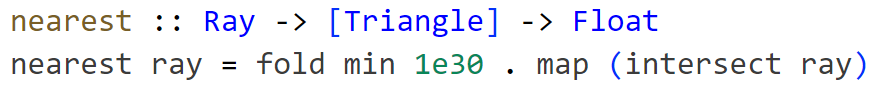
\includegraphics[scale=0.45]{CodeIntro1.png}
\end{figure}

A single ray is intersected with a collection of triangles, where the distance to the nearest triangle is computed by folding over all distances.
As example, an equivalent C-like pseudocode implementation has to take in account both the parallel distribution of work but also the potential vectorization in the inner loop.
As the number of triangles might not be nicely divisible the remaining scalar case must also be handled.
The example is far from optimal as it does not enforce blocks of equal size, but demonstrates the complexity of even a simplified version.

\begin{figure}[ht]
    \hspace{1em}
    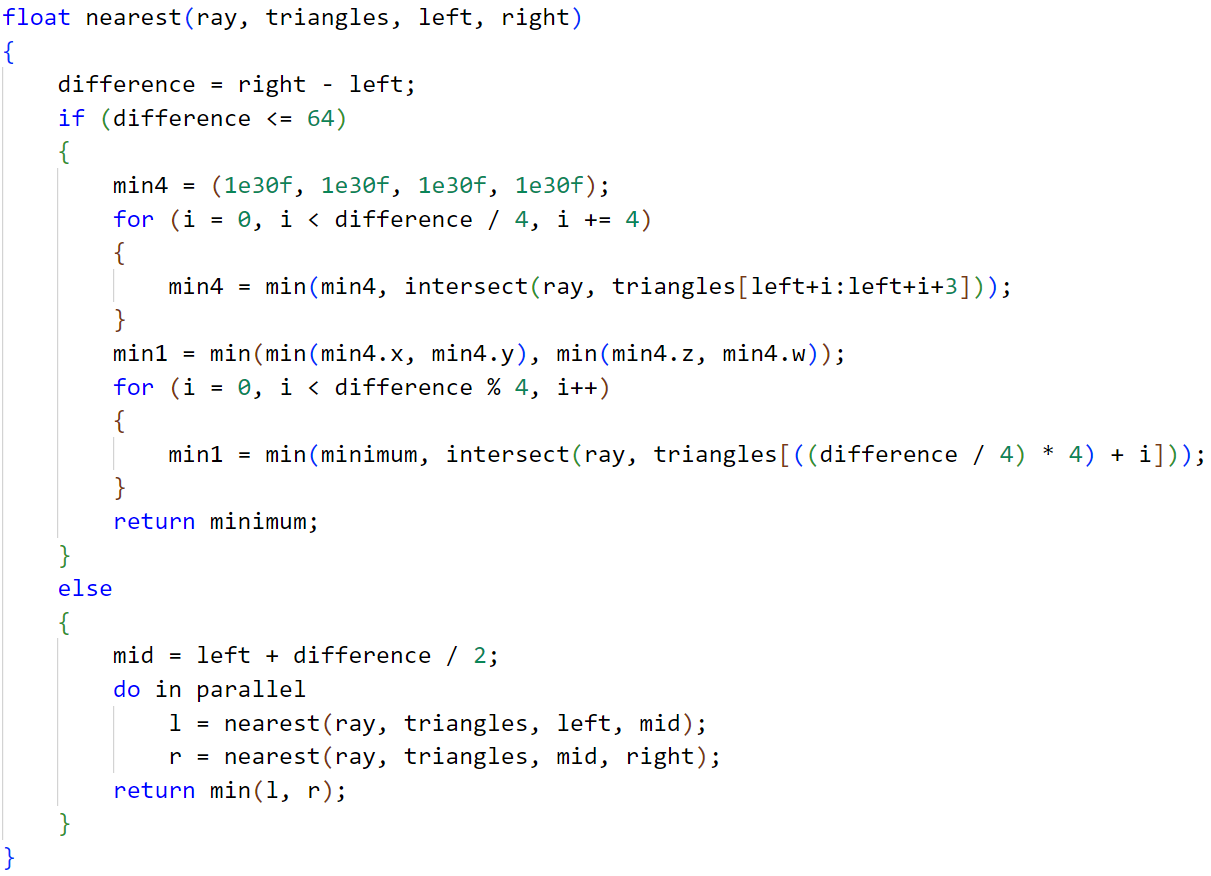
\includegraphics[scale=0.45]{CodeC.png}
\end{figure}

The collective array operations are preferable for both maintainability and expressiveness.
A drawback for working on a higher-abstraction level is the lack of low-level control, which can be crucial in performance sensitive cases.
Sometimes it is easy to incorporate optimizations, with the example of the \type{nearest} function using the sentinel value \type{1e30f} to avoid implementing an explicit failure state.
Making the failed intersection explicit requires branching after each intersection, which hinders data-parallelism in the general case.

\newpage

In other cases this is significantly harder, such as implementing low-level optimizations around memory representation and cache efficiency.
This is apparent when attempting to extend the intersection function to operate on other geometrical shapes, such as spheres.
The most straightforward approach is to create a datatype that can either be a triangle or a sphere.

\begin{figure}[ht]
    \hspace{1em}
    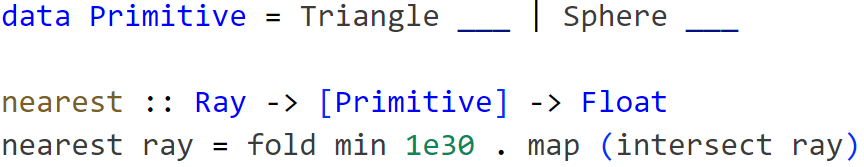
\includegraphics[scale=0.4]{CodeIntro2.png}
\end{figure}

In the general case this will hinder data-parallelism as it requires branching on the identity of the object.
A solution is to store each primitive in their own respective collection.
Static polymorphism is used to define an intersection function for each primitive separately.
Each primitive is folded over separately and later the result of other primitive intersections are combined.

\begin{figure}[ht]
    \hspace{1em}
    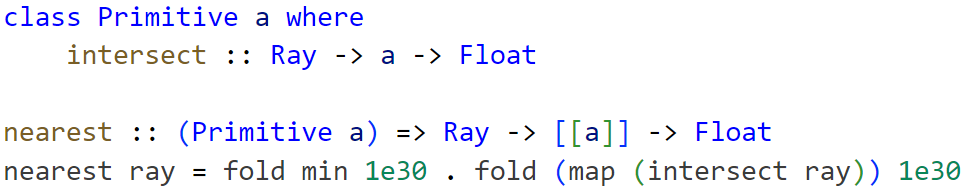
\includegraphics[scale=0.45]{CodeIntro3.png}
\end{figure}

The purpose of both approaches is the same, namely to operate on a collection of primitives.
While we improved the possibility for data-parallelism, we still need to maintain the \type{Primitive} datatype when we want to explicitly return the exact primitive which was intersected with.
To improve our naive ${O}(n)$ implementation we can use an acceleration structure to eliminate primitives prematurely based on their spatial properties.
This means intersections will be performed in smaller batches, to be able to exit early, which reduces the opportunities for data-parallelism.
From a performance standpoint it might be preferable to separate the primitives on a batch-level, requiring even another datatype.
Maintaining the architecture around all these different constructs is ergonomically not viable and caused by our attempt to achieve low-level control.  
A type-safe and generic implementation is often not possible, as both datatypes and interfaces must be defined at compile time.
To remain flexible without explicit defining each representation requires the data to be (re)interpreted at runtime, which breaches type-safety. 
It is also not feasible to manually define mappings between all these different representations.
The inability to abstract over both value-level variant types and type-level variant types prevent a generic higher level abstraction from taking form.

\begin{figure}[ht]
    \hspace{1em}
    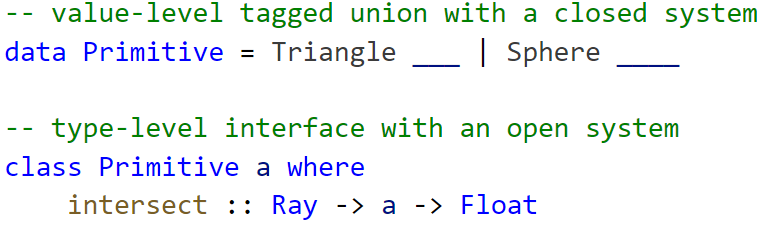
\includegraphics[scale=0.45]{CodeIntro4.png}
\end{figure}

Unifying these concepts allows a collection of primitives to be fully agnostic to the underlying representation.
In this thesis, I propose a transparent way to switch between representations for collections of variant types.
It provides the convenience of an high-level abstraction, while being able to capture the relevant low-level optimizations. 
Type-safety is preserved by elevating the concept of a mutually exclusive datatype to the type-level, which is achieved through type-level and datatype-generic programming.
This way, the easy to use surface-level datatype is mapped automatically to an efficient machine-level representation. 
The machine-level representation, as well as efficient (de)construction can be specified in detail and optimized for a particular architecture and application.

It can be utilized by libraries, frameworks and embedded domain-specific languages that exist in languages that facilitate type-level programming and datatype-generic programming, like Haskell.
This control over the memory representation is invaluable for adapting to cache behavior without having to change the architecture around it.
Manual control over the (de)construction also prevents the need for the explicit sentinel value in our intersection algorithm.
The failure state \type{Miss} can be used, which is internally represented as \type{1e30f}.
The \type{min} function uses the value directly while other functions must pattern match on the value \type{1e30f}.
Within the context of raytracing this other function might spawn an extension ray that simulates the ray bouncing of a surface.
Pattern matching on the \type{1e30f} value will limit data-parallelism for all subsequent extension rays.
A solution can be to unconditionally execute like with the \type{min} function or eliminate all rays that failed for each iterative step. 
The latter can now be represented as an internal reorganization in the proposed implementation, as it does not change the identity of the collection but merely the layout and thus no architectural changes are required to support such an optimization.
To summarize, the research questions answered in this thesis are:

\begin{itemize}
    \item How to obtain low-level control that is applicable for high performance computing, while preserving the higher-abstraction surface representation?
    \item What is the conceptualization of a higher-abstraction variant type, which can exercise the obtained low-level control within in a data-parallel environment?
\end{itemize}

\noindent
Concretely, the contributions of this thesis include: 

\begin{itemize}
    \item An extendable deduplication algorithm for the memory representation of a variant type.
    \item Datatype-generic derivation of an isomorphic mapping between any two datatypes.
    \item A collection of multiple variants that can be completely agnostic to its internal representation
\end{itemize}

\subsection{Related Work} \label{related-work}

First the performance considerations must be understood, to capture the most relevant low-level optimizations.
This induces the need for a flexible and type-safe interface around these optimizations, which will be done through type-level and datatype generic programming.
Relevance is established by an implementation in the data-parallel language Accelerate, which is deeply embedded within Haskell.

\paragraph{Performance}\label{performance}

Capturing low-level optimizations in high-level languages can be done through various methods; such as compiler optimizations\cite{compiler-optimization}, a Foreign Function Interface\cite{ffi}, compiler intrinsics or embedded domain-specific languages\cite{accelerate-llvm}. 
For data with multiple representations in a high-performance environment it often involves resorting to untyped code and bitwise operations, to gain control over the memory representation and (de)construction of the variant type.
In data-parallel applications primitive types are distributed over multiple arrays to facilitate vectorization.
It is not apparent what the representation of a tagged union should be\cite{accelerate-sum-types}, as they inherently break vectorization in most cases. 
The functional data-parallel languages Accelerate\cite{accelerate-sum-types} and Futhark\cite{futhark-sum-types} implicitly distribute primitive types in composite datatypes over multiple arrays.
Both implementations have limited deduplication capabilities, but research has been done to integrate a memory efficient tagged union in Accelerate\cite{accelerate-sum-types}.
Game-engines, which deal with many clusters of data, have a fundamentally different approach as they have widely adopted the Entity-Component-System (ECS) pattern\cite{ecs-origin}. 
Many implementations; such as Unity\cite{unity-ecs-patent}, Flecs\cite{ecs-flecs} and Bevy\cite{ecs-bevy}, incite a collective reorganization of data when a variant change occurs at runtime.
A type-safe and performant implementation is notably hard, as all interactions between the representations must be statically resolved.
More generally, research on zero cost abstractions over memory representations are prevalent in C++ libraries such as LLAMA\cite{llama} and Alpaka\cite{alpaka}. 

\paragraph{Interface}

Functional languages handle tagged unions safely through Algebraic Data Types (ADTs), where sum types categorize ADTs with multiple variants.
Constructors can be local to an unique ADT (nominally typed) or exist as independent types (structurally typed).
Deconstructing is done by pattern matching, where functions natively branch on the current active variant.
In Haskell sum types are nominally typed, which means variants are not standalone types and cannot exist safely outside the ADT.
Structural sum types are often called extensible or open sum types, as they do not have to be explicitly declared before use.
In OCaml these are natively supported as polymorphic variants\cite{polymorphic-variants}, while Futhark is completely structurally typed and refers to them as sum types\cite{futhark-sum-types}.
Deriving a memory representation for user-defined datatype can be done statically through type-indexed types\cite{type-indexed}\cite{associated-types}.
In C++ these are called {\it traits}\cite{c++traits} and in Haskell these are called {\it type families}\cite{type-families}. 
As stated earlier, some C++ libraries also attempt to create zero cost abstractions around memory representations\cite{llama}\cite{alpaka}.
Datatype-generic programming\cite{datatype-generic-programming}, which parametrizes on the composition of a datatype, can be used to create mappings between the derived representations.
Both concepts are used in highly generic libraries for a wide-range of applications\cite{generic-programming}. 

\paragraph{Implementation}

Variant types are rare in array languages, likely due to a combination of the infrequency of non-uniform data in data-parallel applications and the required low-level control in the instances they are needed.
The functional array languages Accelerate and Futhark have only recently gotten support for sum types\cite{accelerate-sum-types}\cite{futhark-sum-types}.
Accelerate is a data-parallel array language deeply embedded within Haskell, where sum types are currently represented as a non-compact tagged union.
Research has been done on a compact tagged union representation for parallel arrays in particular, which has been named a {\it Recursive Tagged Union}\cite{accelerate-sum-types}.
The representation uses a unified tag for nested sum types, which optimizes memory usage at the cost of tag (de)construction but has not yet been integrated within Accelerate. 
Futhark is a functional structurally typed data-parallel array language, where the sum types only deduplicate identical primitive types.
The research pertains primarily to including structural sum types to the Futhark compiler\cite{futhark-sum-types}, rather than performance.

\newpage

\section{Background}\label{background}

There are many components that can influence the performance of a program.
This increases the importance of being able to identify {\it bottlenecks} but also understanding the underlying technological performance considerations.
The first subsection introduces fundamental optimizations related to the interaction between data and hardware are introduced.
This is used to identify architecture agnostic performance considerations for operations on collections of data in the second subsection.
In the third subsection this information is used to discuss efficient data structures for multiple variants of a type.

\subsection{Optimizations}\label{optimizations}

In the early days of computing, memory was seen as a way to store data indefinitely.
As computational power of processors increased, the importance of main memory increased.
Main memory is dependant on the advancements of random-access-memory (RAM), which stagnated due to both cost and physical limitations\cite{memory}. 
This put pressure on the software side to adapt to hardware components for optimizations, rather than merely the computational complexity of algorithms.
One of these hardware optimizations is cache storage, which accelerates memory accesses of predetermined data.
The chosen data is decided based on a cache replacement policy, often based on a temporal property. 
The cache operates independently of the operating system\cite{memory}, and no direct control can be exercised.

\begin{figure}[ht]
    \centering
    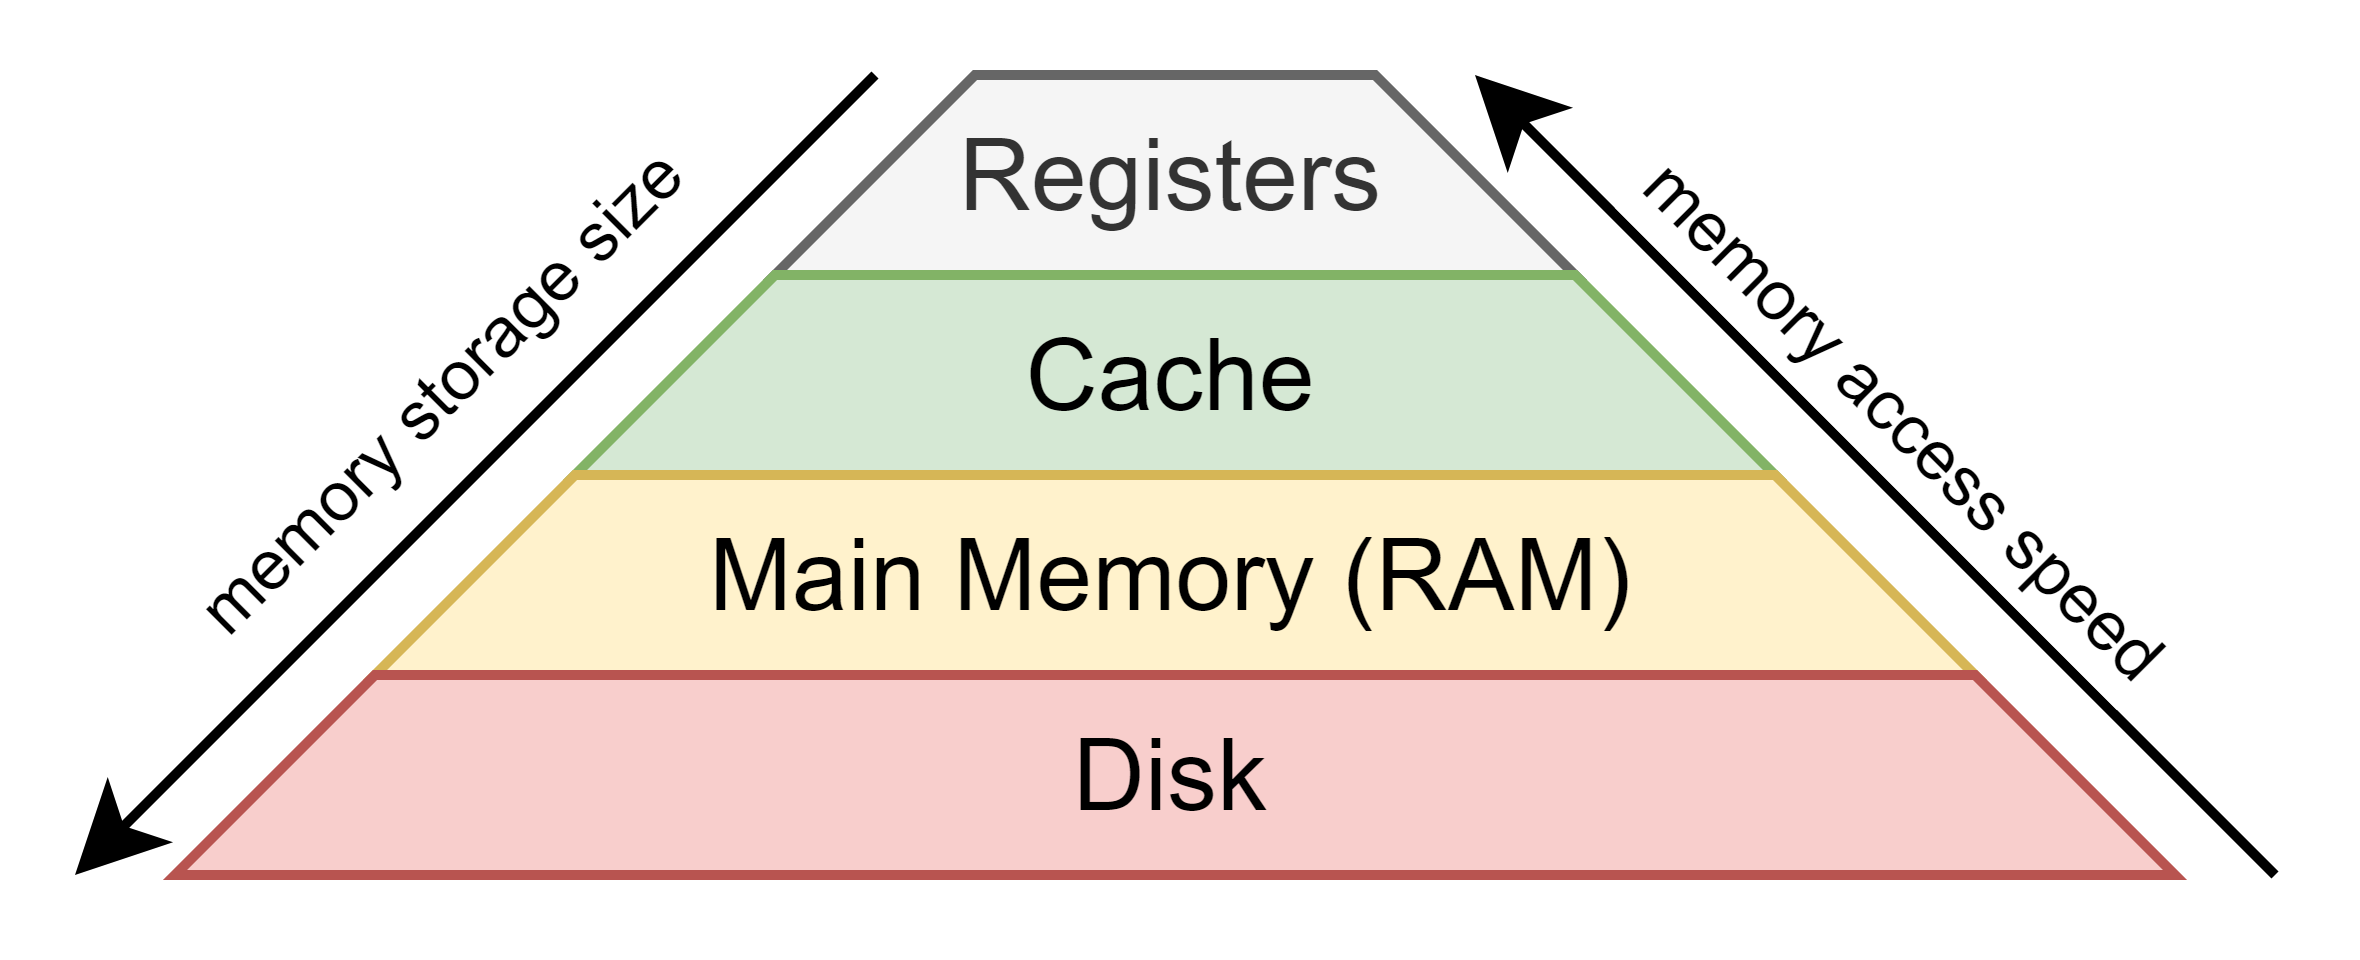
\includegraphics[scale=0.10]{Performance1.png}
    \caption
    {
        An abstract view of a computer memory hierarchy. 
        Each layer can be subdivided even further, depending on the type of hardware. 
        The difference between both the memory access time and memory storage size for each layer can be several order-of-magnitudes.
        As example: data in a register effectively takes 0 instruction cycles, while data from disk might take several million instruction cycles to arrive.  
    }
\end{figure}
\paragraph{Instructions}

Interfacing with processors is done through computer instructions.
Fetching of an instruction is a memory operation in itself, as it retrieves the instruction at the target of the program counter.
Instructions operate on registers, which have distinct sizes depending on the architecture and their respective function.
There are many instruction set architectures (ISA) and devices that utilize only a specific instruction set.
An intermediate representation (IR), such as the LLVM IR\cite{LLVM}, can be used to create a single interface for multiple instruction sets\cite{intermediate-representation}.
Hardware design sometimes allows for specialized instructions\footnote{Note that this is separate from a {\it complex instruction}, which concerns a compact {\it representation} of several instructions. }, such as square root approximations, which are faster than their semantically equivalent instruction(s).
Other examples include sacrificing accuracy for performance (floating-point), combining a sequence of instructions (arithmetic) or by parallel execution on multiple data elements (SIMD).
SIMD instructions in particular are often very performant, as several steps within the execution pipeline can be parallelized.
The process of parallelization of multiple instructions is called {\it vectorization}.
Using these architecture dependant instructions directly can be achieved through compiler intrinsics.

\begin{figure}[ht]
    \centering
    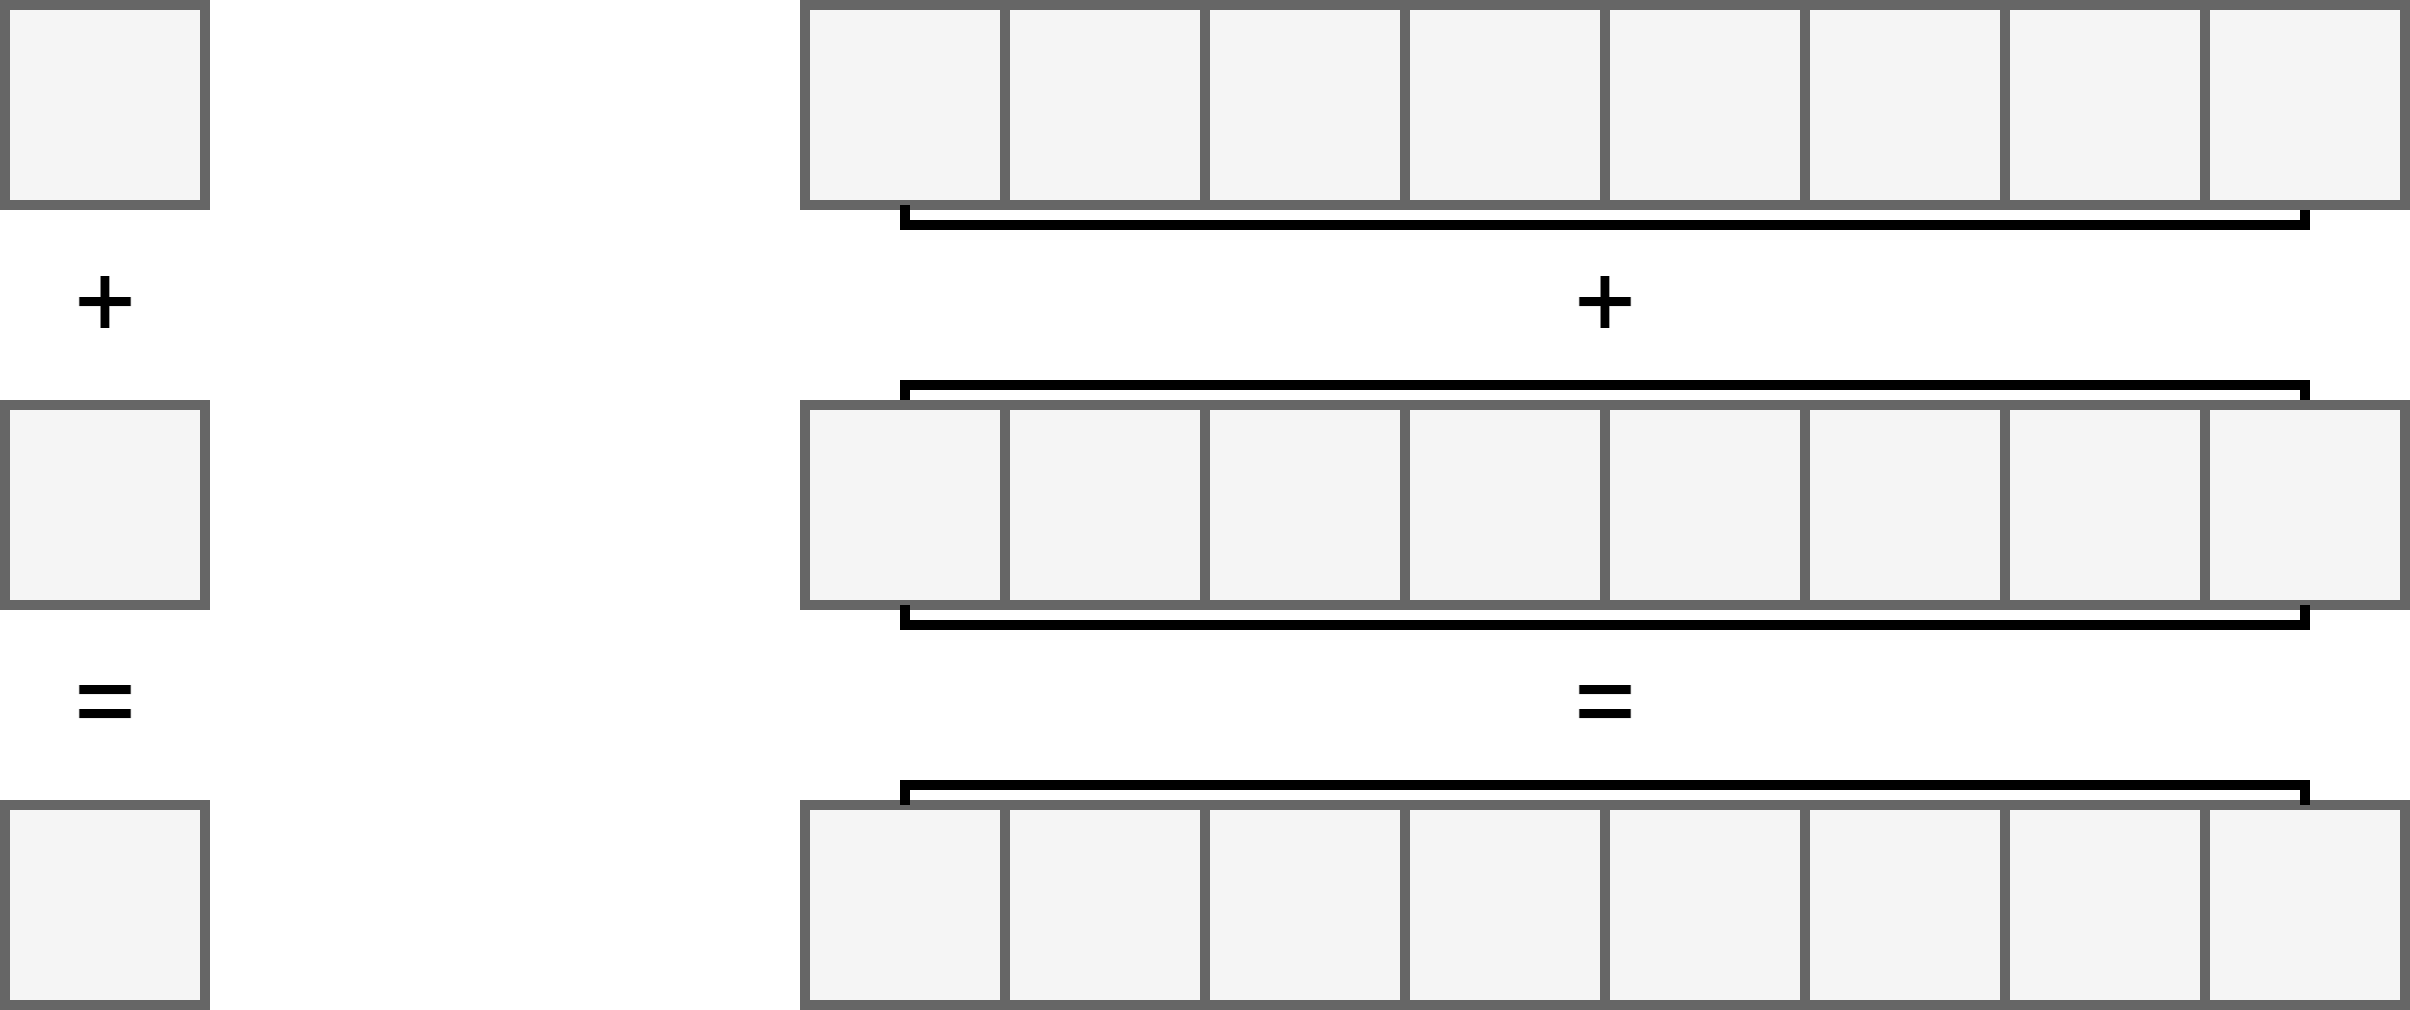
\includegraphics[scale=0.1]{Performance2.png}
    \caption
    {
        A scalar addition instruction is converted to the equivalent single instruction multiple data (SIMD) instruction, where each grey square denotes a single data component.
        Vectorization requires the data to be contiguous in memory and effectively performs the work of several scalar operations within a single instruction.  
    }
\end{figure}

\newpage

\paragraph{Register Pressure} 

Registers can be considered the fastest available memory, as the data is ready to be used by an instruction.
Within the context of registers this data is commonly referred to as a variable.
Variables being preloaded into registers before execution is a prerequisite for reasonable performance.
The scheduling problem of ensuring all variables exist in registers before execution is to be considered a NP-complete problem\cite{register-allocation}.
Programming languages with any form of abstraction generally delegate this process to the compiler.
It simplifies a lot of complexity, as only which data is being used by what instruction is relevant for the programmer.
In some cases there are too many live variables for the available registers, which can {\it spill} the variable.
This requires a variable to be stored outside registers, in a slower form of memory, and incites a delay when attempting to use the data.
It can be prevented by either reducing the time variables are live, reordering the sequence of instructions or diversifying the execution units.  

\paragraph{Memory Access Time}

Semantically random-access-memory (RAM) implies that memory operations take around the same amount of time, independent of the physical storage location.
In practice this does not hold for several reasons.

\begin{itemize}
    \item [SRAM/DRAM]
    On a modern system there often exist several different types of RAM, mostly driven by cost differences.
    The main forms of RAM are static RAM (SRAM) and dynamic RAM (DRAM).
    SRAM uses six transistors to represent a single bit, while DRAM only uses one transistor with a single capacitor. 
    A capacitor loses electrons over time which means data has to be refreshed repeatedly to preserve its data.
    A refresh requires both read and write operations, which interferes with other memory operations.
    This makes DRAM inconsistent and on average significantly slower but much cheaper to produce due to requiring less transistors\cite{memory}.

    \item [Propagation]
    Data is transferred by using electrical charges through semi-conductors.
    This creates a physical limitation dictated by physical distance and temperature.
    This is called propagation delay and poses a hard limitation to the rate at which components can operate on.
    SRAM is often located physically closer to the execution units to utilize the faster memory access more effectively.
 
    \item [DMA]
    A processing unit needs to forward the requested data to the targeted location, which takes up processing time.
    Direct-memory-access (DMA) is an interface for hardware components and allows memory operations to be more organized.
    This allows for large scale memory operations to be performed efficiently and independently of the main processor.
    It requires use of several buses which means some processors must idle at seemingly random periods of time.
    In essence it means that other hardware components can influence the memory access time.
\end{itemize}

\newgeometry{bottom=0.5cm}
\newpage

\paragraph{Caching}

Due to the hardware related discrepancies between memory access time, which we discussed in this subsection, it can be beneficial to organize data according to the memory access time.
The simplest way to achieve this is by caching data, that is storing a {\it copy} of the data in a faster accessible medium.
A cache generally consists of SRAM and resides close to the processor, which allows memory accesses to be order-of-magnitudes faster than a main memory access\cite{memory}.
When data already exist in the cache it is referred to as a cache hit, otherwise a cache miss has occurred.
Deciding which data is cached and for how long is a cache replacement policy, utilizing both recency and frequency.
Adapting to policies simplifies both the scheduling and minimizes the potential cache misses that can occur in the worst case scenario.

\begin{figure}[ht]
\begin{minipage}{.65\textwidth}
Caching of data can be done after the data has already been retrieved, which means a delay already has occurred.
This can be avoided by requesting data in advance and storing the data in a cache prematurely, so called cache {\it prefetching}.
It can be accomplished by analyzing future instructions (hardware) or using instructions that {\it hint} at the future use of a piece of data (software)\cite{cache-prefetching}.
Prefetching is harder when there are multiple execution paths possible, as both the data and the next instructions will be uncertain.
Speculatively executing the uncertain instructions can be performant if the overhead of redundant work remains small enough.
Rather than executing unconditionally, some processors execute the most likely to happen branch based on some parameters (branch prediction)\cite{instruction-level-parallelism}.
\end{minipage}%
\begin{minipage}{.35\textwidth}
    \centering
    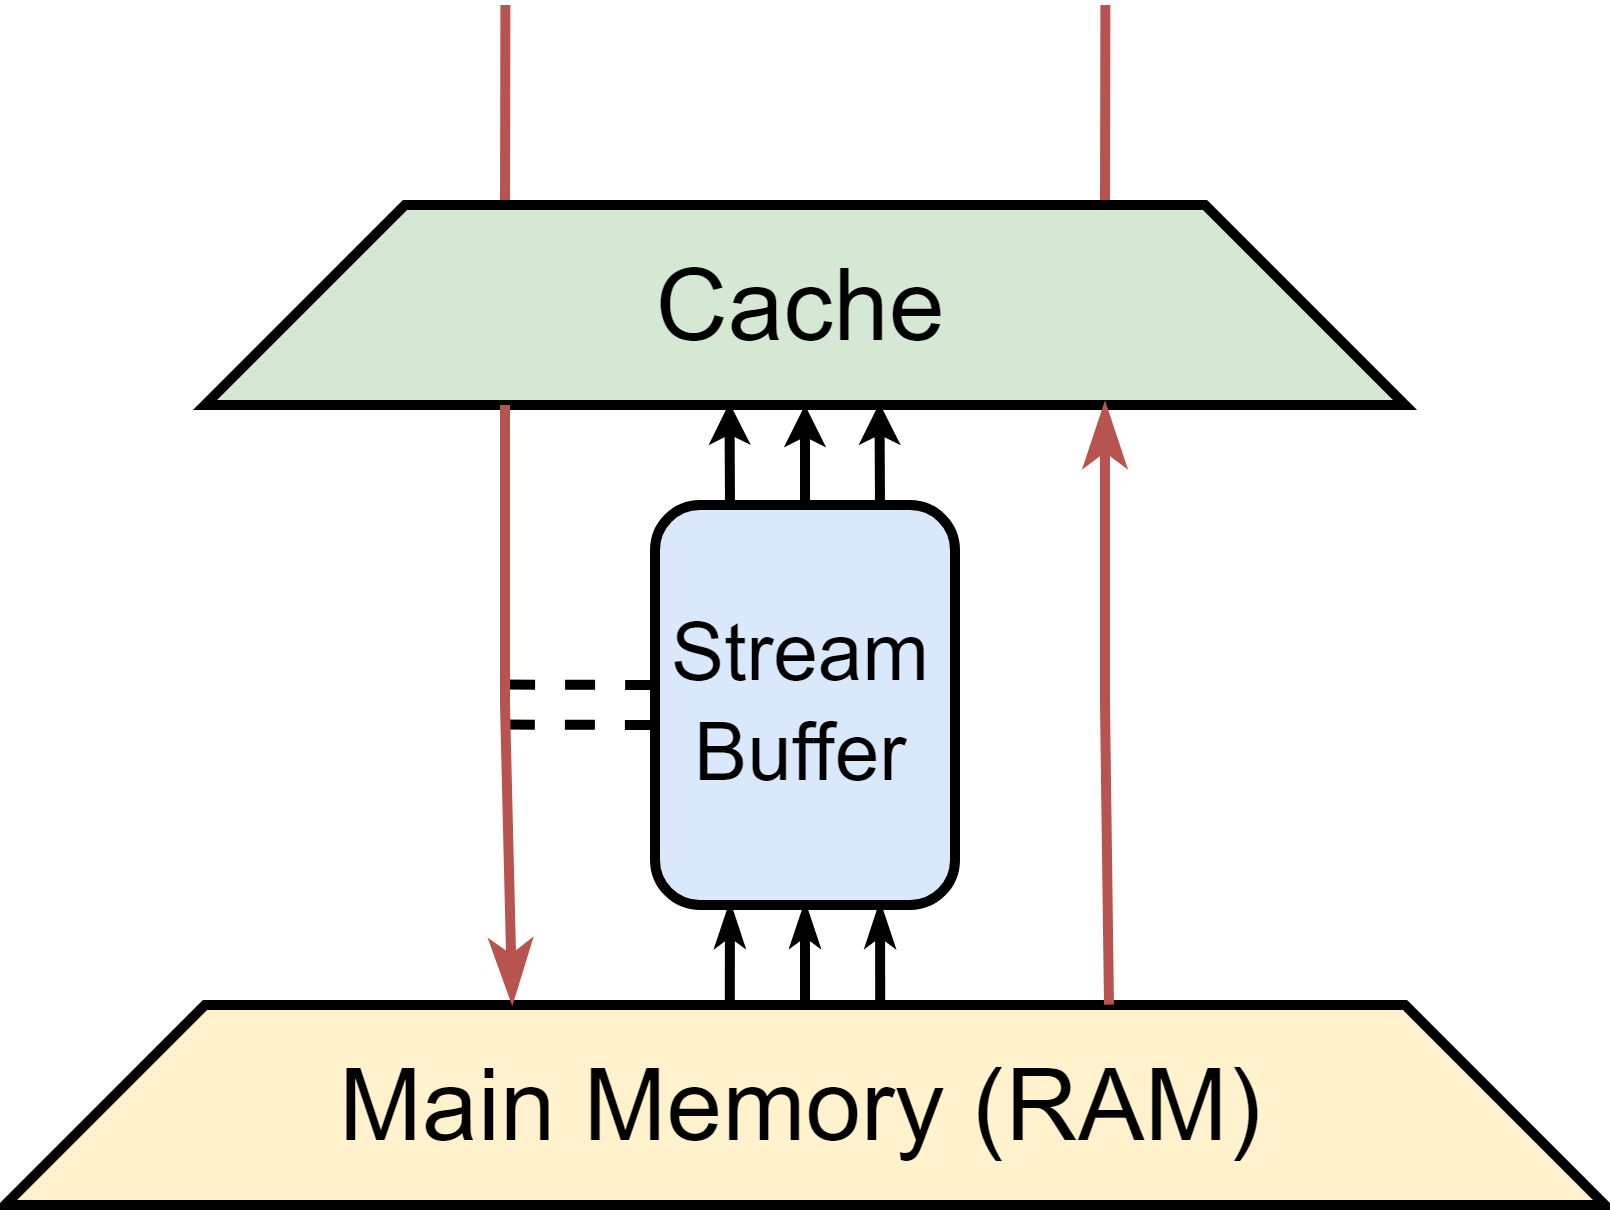
\includegraphics[scale=0.08]{Performance3.png}
    \captionsetup{margin=0.5cm}
    \captionsetup{format=plain}
    \caption{Stream buffer that prefetches data into the cache based on cache misses.}
\end{minipage}
\end{figure}

\vspace{-1.5em}

\paragraph{Parallelism}
Instruction-level parallelism is the parallel execution of multiple instructions\cite{instruction-level-parallelism}.
It can be done by dividing an instruction into several steps and outsourcing each step to a distinct processor unit (instruction pipelining).
Shuffling the order of instructions might allow more units to work in parallel from each other (out-of-order execution).
This can be extended by outsourcing instructions to different units of the same type, such as execution units (superscalar execution).
An abstraction-level higher is data-level parallelism, which executes a single instruction on multiple data elements such as the previously discussed SIMD instructions.
Specialized processors sometimes either fully pipeline the data (vector processing) or allow for some form of autonomy (multithreading). 
Both share instruction fetching and decoding, but threads have their own program counter which allows for an independent sequence of instructions.
Execution of threads can be done concurrently, which can be useful to hide latencies (context-switching).
In parallel is also possible with multi-core processors, which have several processors units (cores) that can support multiple threads at the same time.
Cores are often not independent processors and might share several components with other cores, such as caches\cite{thread-level-parallelism}.

\begin{figure}[ht!]
    \centering
    \begin{minipage}{.5\textwidth}
        \centering
        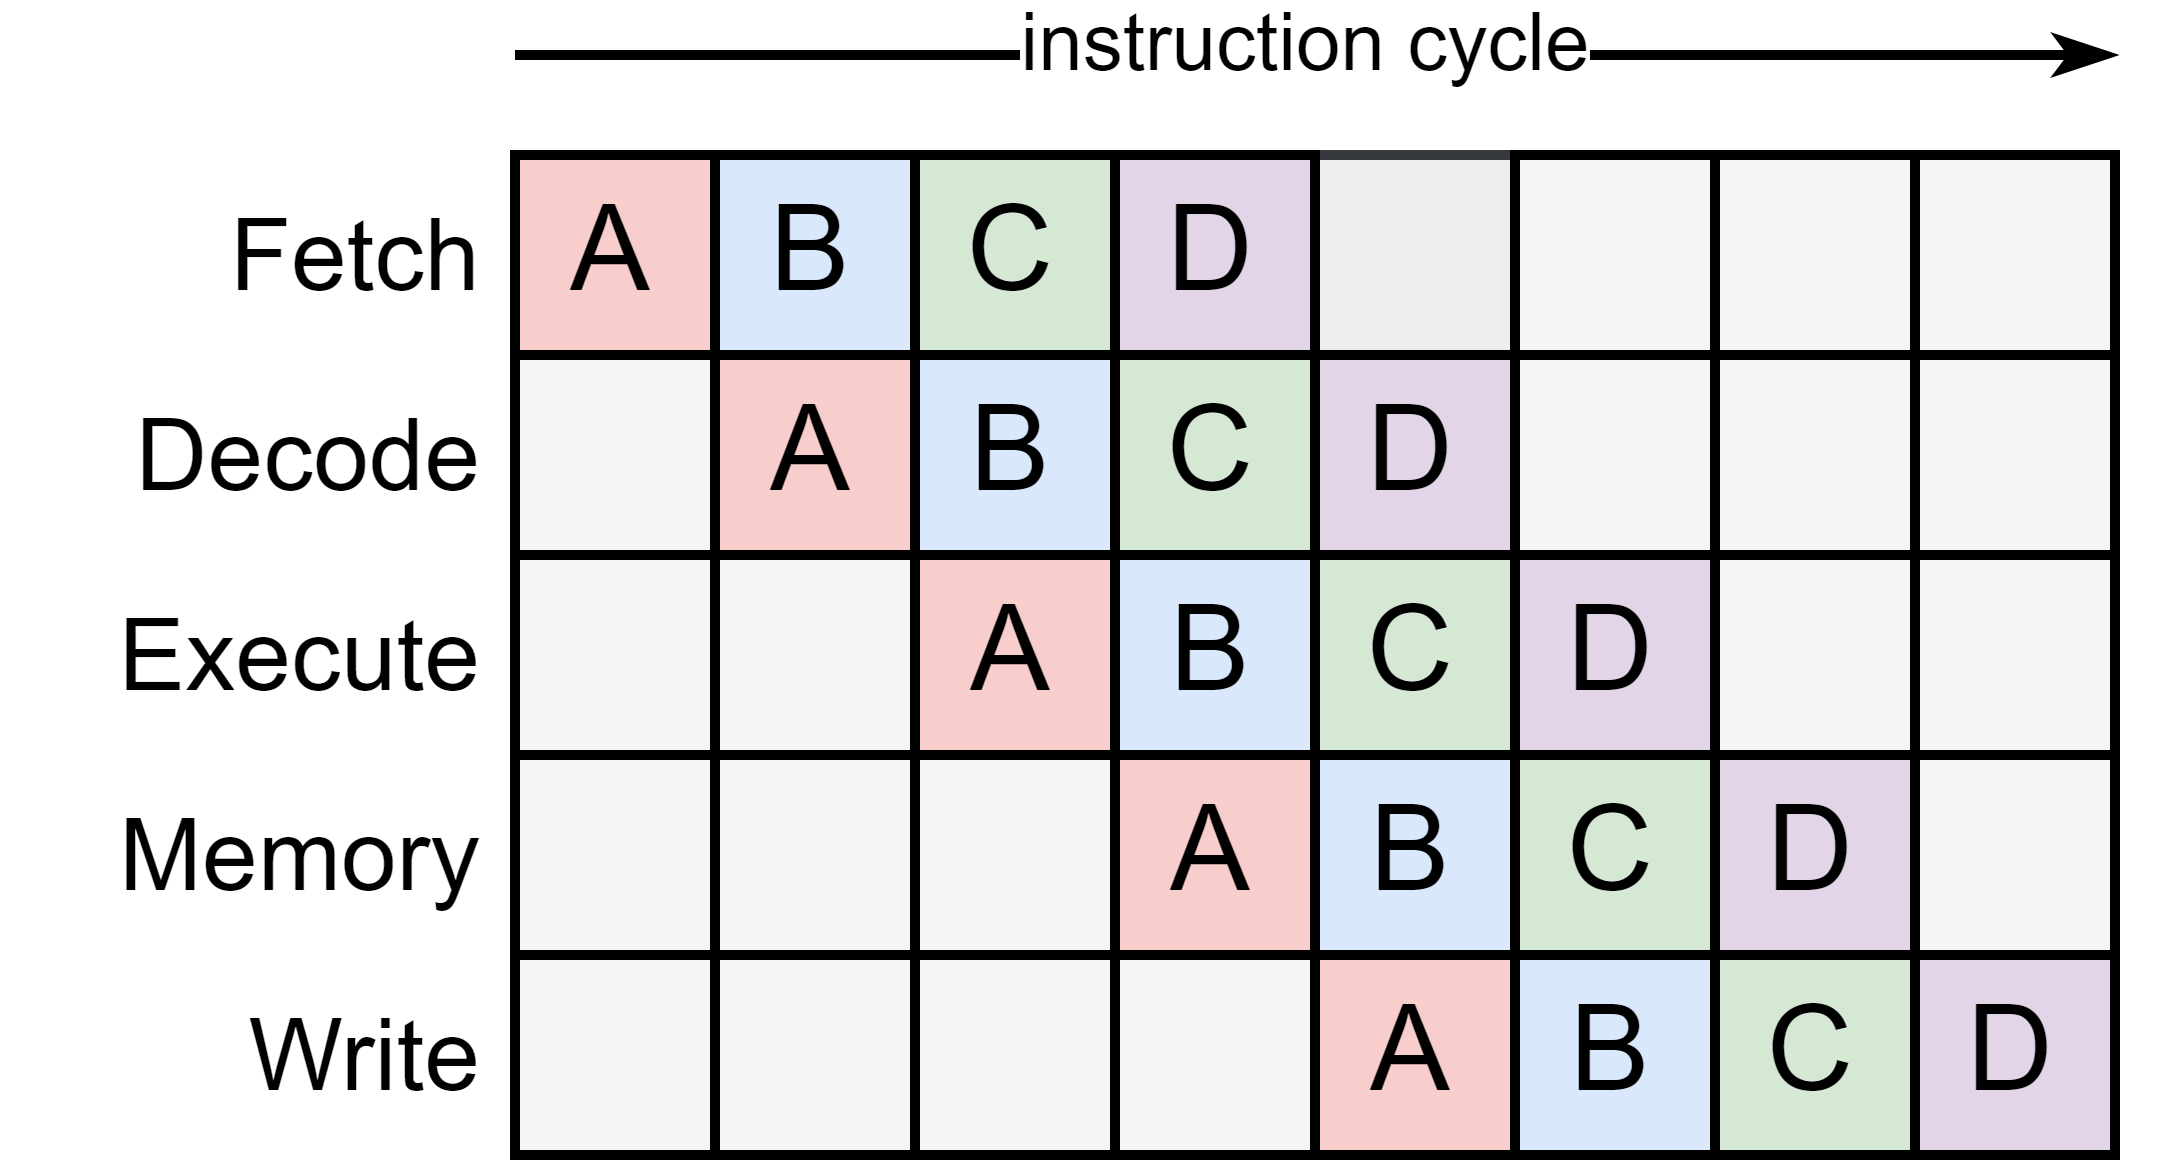
\includegraphics[scale=0.09]{Performance4.png}
        \captionsetup{margin=0.2cm}
        \caption
        { 
            Multiple phases allows a processor to hypothetically execute the [A, B, C, D] instructions in 8 cycles.
            This is significantly faster in comparison to the 20 cycles it would require in a single lane.
        }
    \end{minipage}%
    \begin{minipage}{.5\textwidth}
        \centering
        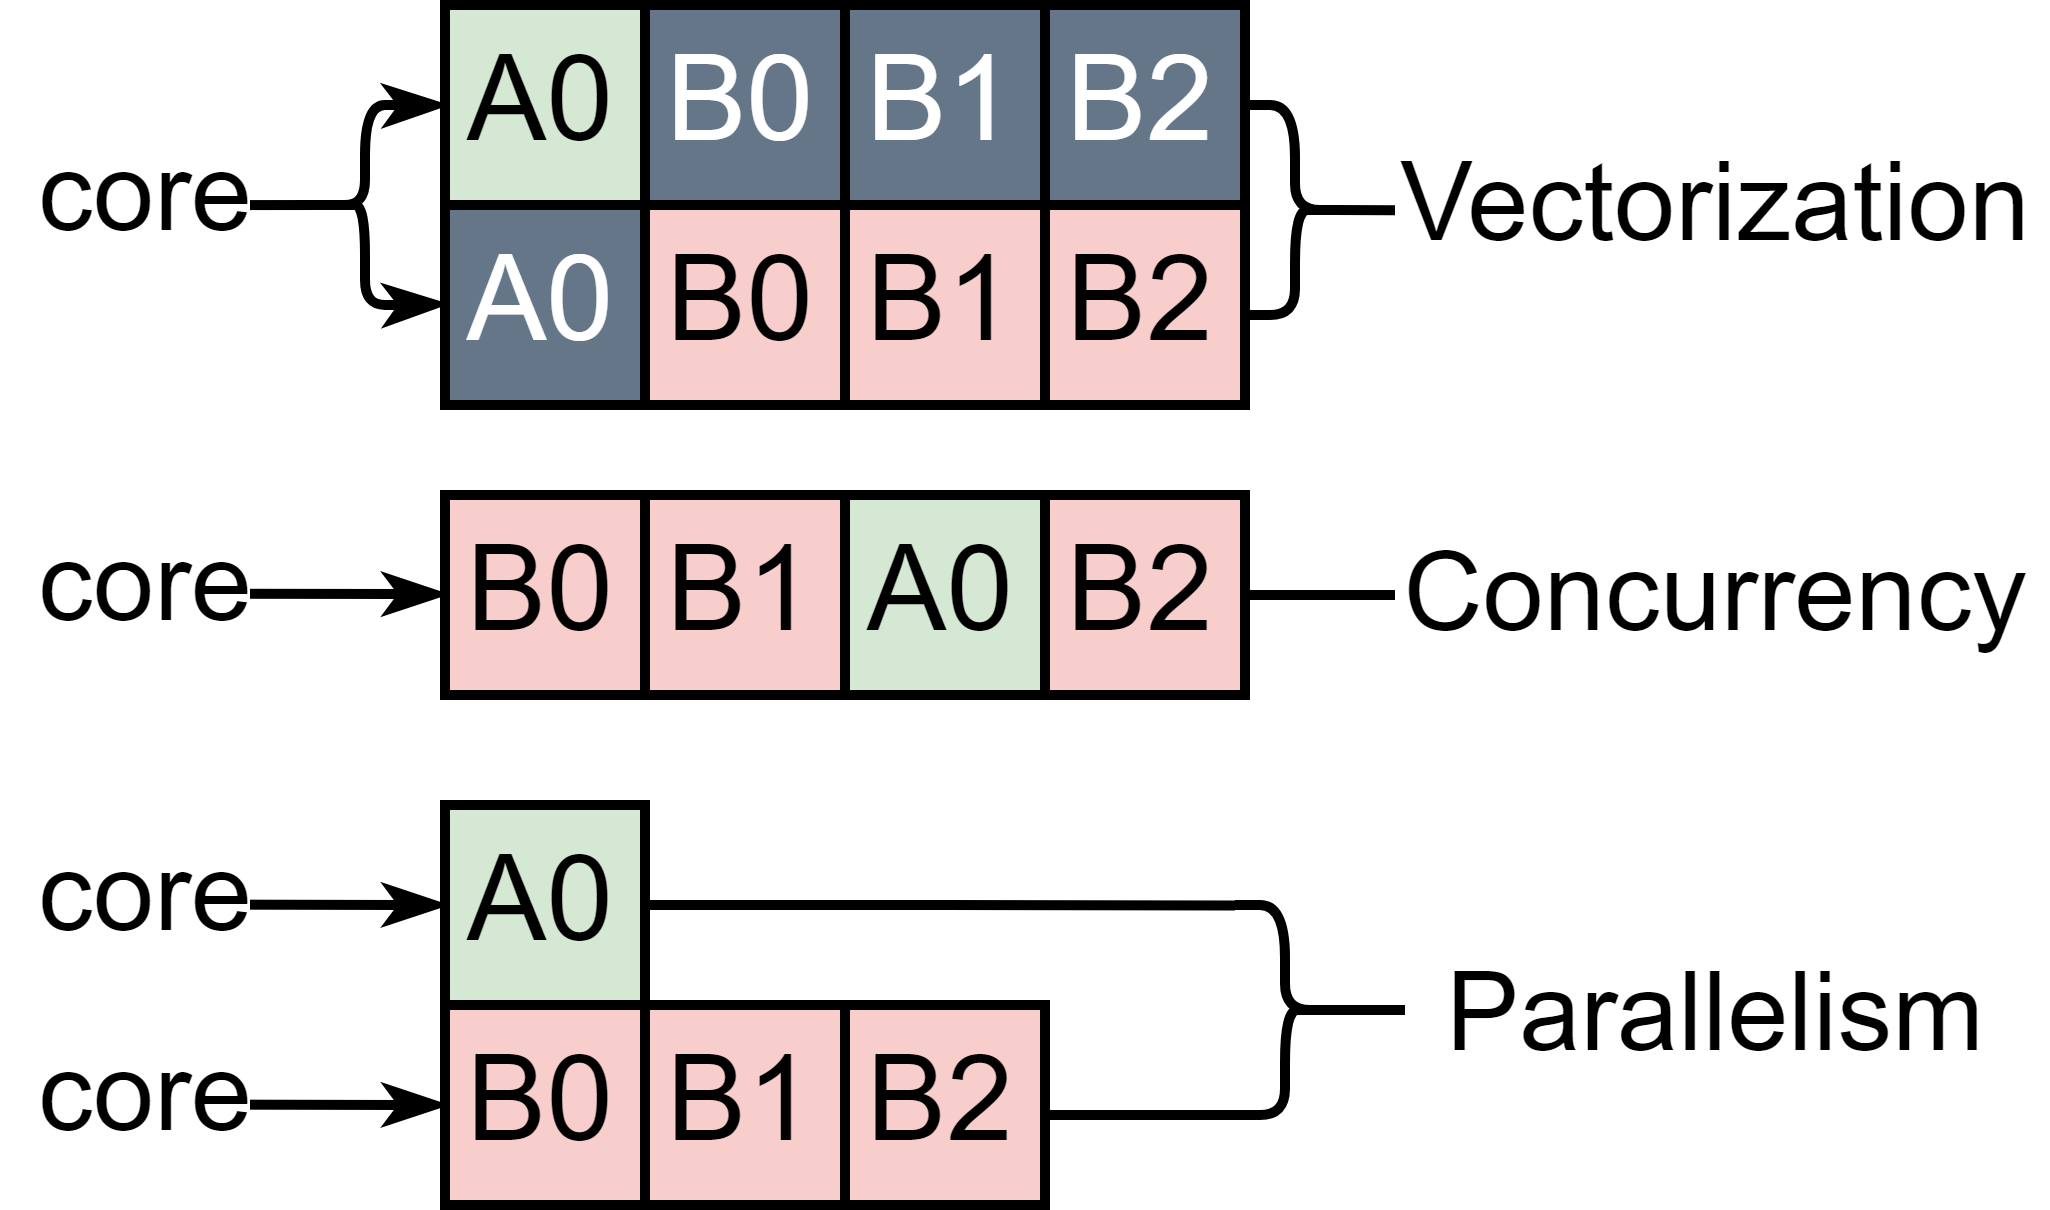
\includegraphics[scale=0.09]{Performance5.png}
        \captionsetup{margin=0.2cm}
        \caption
        { 
            Both vectorization and concurrency are single lane concepts, but differ in handling multiple tasks.
            Parallel threads are both independent and execute on multiple cores simultaneous.      
        }
    \end{minipage}
\end{figure}

\restoregeometry
\newpage

\subsection{Principles}

In the previous section several components have been identified that can influence the performance of a program, such as the cache.
The interconnectivity of the components make general statements on optimizations often weak, as the environment in which the optimization exist can heavily influence the result.
Focusing on a particular area, such as iterating on multiple data elements in parallel, allows for a stronger argument.
Within this section previously discussed intricacies will be discussed in the context of iterating on many elements in parallel.

\paragraph{Contiguous} 

It is beneficial to contiguously allocated data, like an array, so that all elements can be identified in constant time\footnote{Both in {\it time complexity} and within {\it computer architecture} norms, as data access from a memory location consists of a single instruction. This is in contrast with data structures such as pointer trees and hash tables, which require several instructions due to pointer chasing. } through a linear function.
Composite datatypes work similarly, where each field exists as a predefined offset from the base memory location.
Such structure also simplifies work distribution between threads, as all data is segregated through constant offsets.
For vectorization contiguous data is a prerequisite as instructions operate on singular contiguous blocks of data.
If data is not spatial adjacent in memory, data must aligned temporarily or complex interleaving methods must be used\cite{interleaved-SIMD}.
Therefore composite datatypes interfere with vectorization in the general case, as the spatial adjacent data includes fields within the same datatype.
Parallel arrays solve this by creating a distinct array for each primitive type within the composite datatype so that each field within the composite datatype can be vectorized independently.

\begin{figure}[ht]
    \centering
    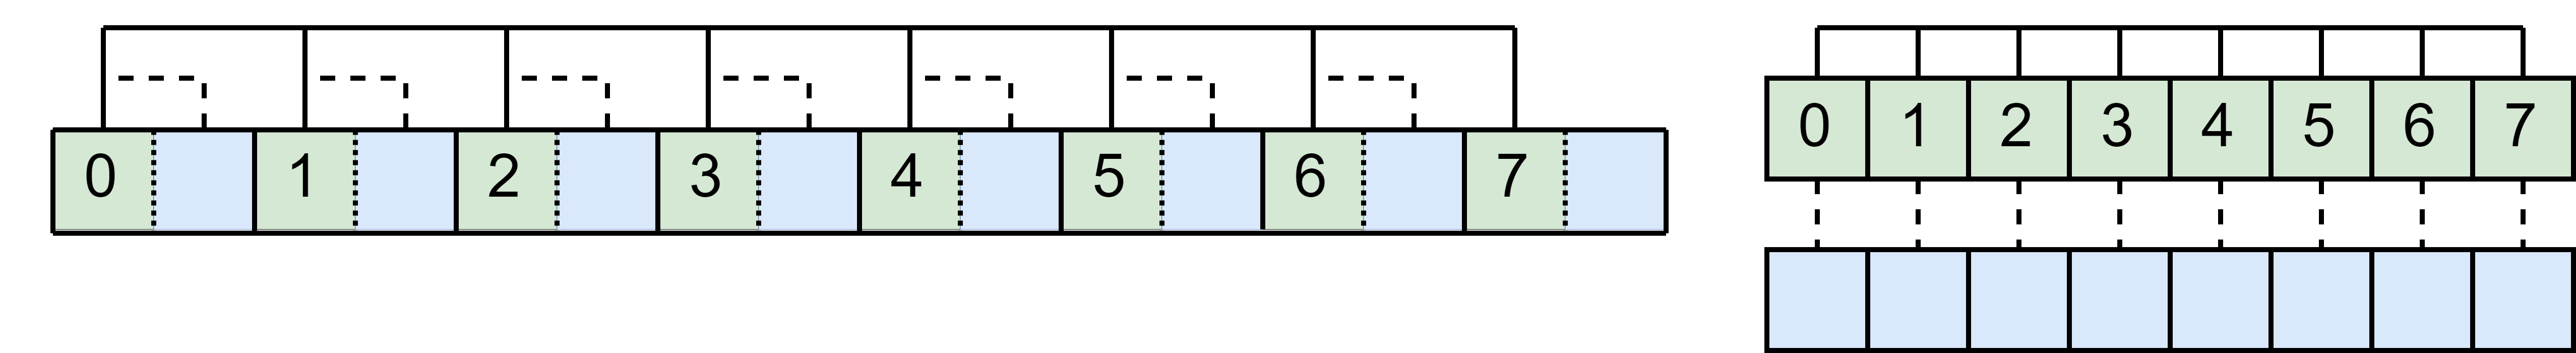
\includegraphics[scale=0.082]{Performance6.png}
    \caption
    {
        Visual comparison between an array-of-struct collection(1) and a struct-of-array collection(2). 
        The solid lines represent indices in an array and the dotted lines denote an implicit connection that is relative to the original index.
    }
\end{figure}

Caches also operate with contiguous blocks of memory, which means spatial adjacent data within a fixed alignment are stored together.
A struct-of-array collection lends itself well to the cache, as it means the least amount of cache blocks are required irrespective of block size and alignment\footnote{Note that this is only the case when {\it all} elements in an array are operated on, which falls under the predefined context of this chapter.}.
A function that operates on a single field in an array-of-struct collection pollutes the cache with the (unused) fields, which is not an issue for the struct-of-array collection. 
In addition all memory accesses use the same linear function, a {\it constant stride} access behavior, which makes it particularly receptive to hardware cache prefetching\cite{cache-prefetching}. 

\paragraph{Access Patterns}

As the cache is finite in size, a cache block can be ejected prematurely.
Both for data within the same cache block but also when the same block is required at multiple times in the application.
As stated in section \ref{optimizations} the cache replacement policy is based on temporal properties, which can be leveraged to increase the chance requested data exists in the cache.
By avoid random accesses and organizing computations around when the data is used we can increase the temporal locality of our application.
This is non-trivial in iterations which access multiple indices (stencils) or computations that inherently involve some random access (linked lists).
Due to the way caches operate with contiguous blocks, spatial locality of data commonly used together can also reduce the total amount of cache blocks that are required. 

\newpage

\begin{figure}[ht]
    \centering
    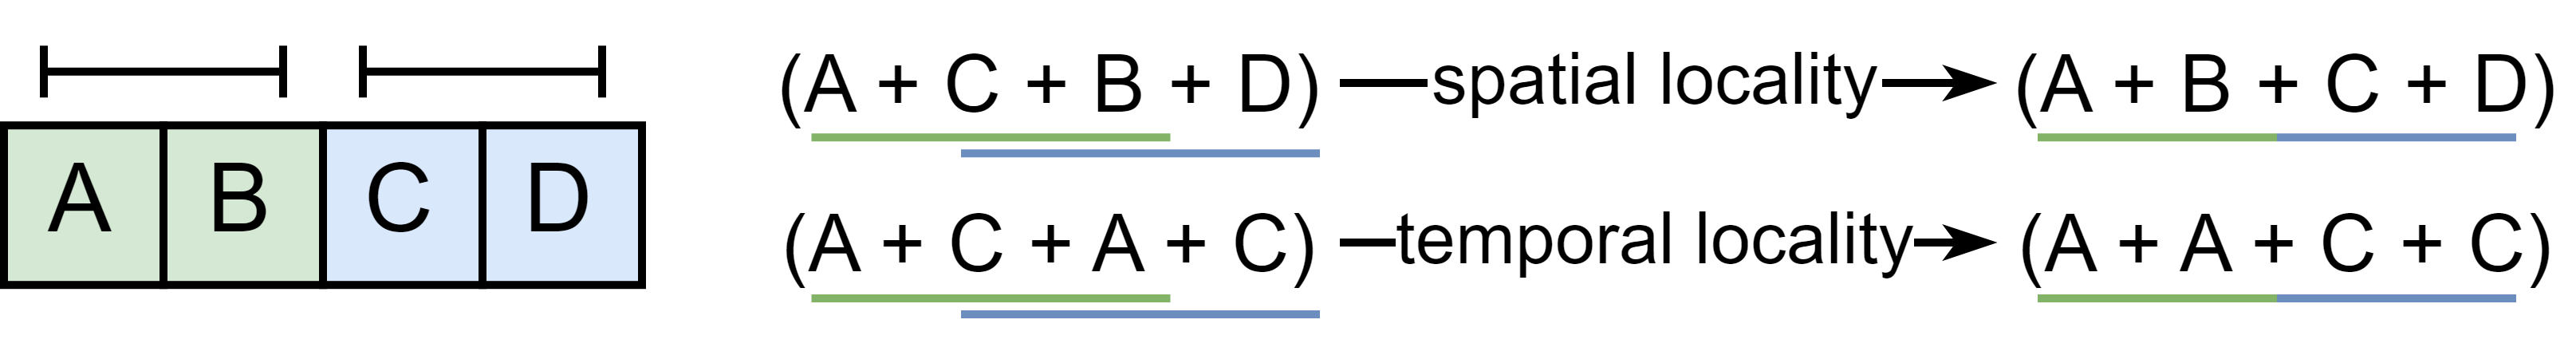
\includegraphics[scale=0.12]{Performance7.png}
    \caption
    {
        Comparison between temporal and spatial locality, where the data A/B and C/D will exist in different cache blocks when stored in the cache.
        The initial sequence of operations has overlapping live time of cache blocks.
        Reordering the operations can facilitate both spatial and temporal locality.
    }
\end{figure}

A way to contextualize this is by considering multiple iterations on an array.
Partitioning the array and iterating on a single segment at a time means cache blocks will be reused (tiling).
Cache coherence can be further improved by also accounting for shared resources, by grouping elements that use the same resource in their instruction sequence. 
This technique is explored in raytracing\cite{raytracing-reorder-ray}, where rays are sorted to exploit the fact that spatially adjacent rays likely traverse the acceleration structure similarly.
Avoiding redundant cache blocks is also important for multi-core processors, as it reduces the need for data to exist in multiple caches at the same time and minimizes cache reloads.

\paragraph{Branching}

Pipelining instructions is not possible when the sequence of instructions is dependant on the result of a previous instruction.
This limits instruction-level parallelism, which is solved through various ways of unconditional instruction executions\cite{instruction-level-parallelism}.
Either by discarding the computed results or by {\it flushing} the pipeline when the wrong branch is predicted, both of which intuitively have an overhead.
A compiler can eliminate\footnote{Either by proofing the branch will never be executed or by replacing the branch with a {\it conditional move} instruction, which only writes the result on true.} branches or move loop-invariant code to facilitate instruction-level parallelism\cite{assembly-optimizations}. 
These optimizations do not always improve performance, as an increase in instructions can pressure registers usage and the cache.  
It is also limited to instructions that cannot fail or overflow, as unconditional execution of these instructions can introduce unintentional side-effects.  

\begin{figure}[ht]
    \begin{minipage}{.5\textwidth}
        Branching is also problematic for vectorization, as all data within the instruction size must follow the same sequence of instructions.
        It can be resolved through the use of a {\it bitmask}, which can nullify parts of a result\cite{assembly-optimizations}.  
        Another notable application of unconditional execution is sequential loops, where unrolling the loop creates an opportunity to vectorize the scalar instructions.
        Automatic vectorization of loops is an active field of research, and limitations have been primarily attributed to the lack of analysis information available to compilers\cite{automatic-vectorization}. 
        This means branchless code and simplifying control flow allows the compiler to vectorize instructions in more instances.   
    \end{minipage}%
    \begin{minipage}{.5\textwidth}
        \centering
        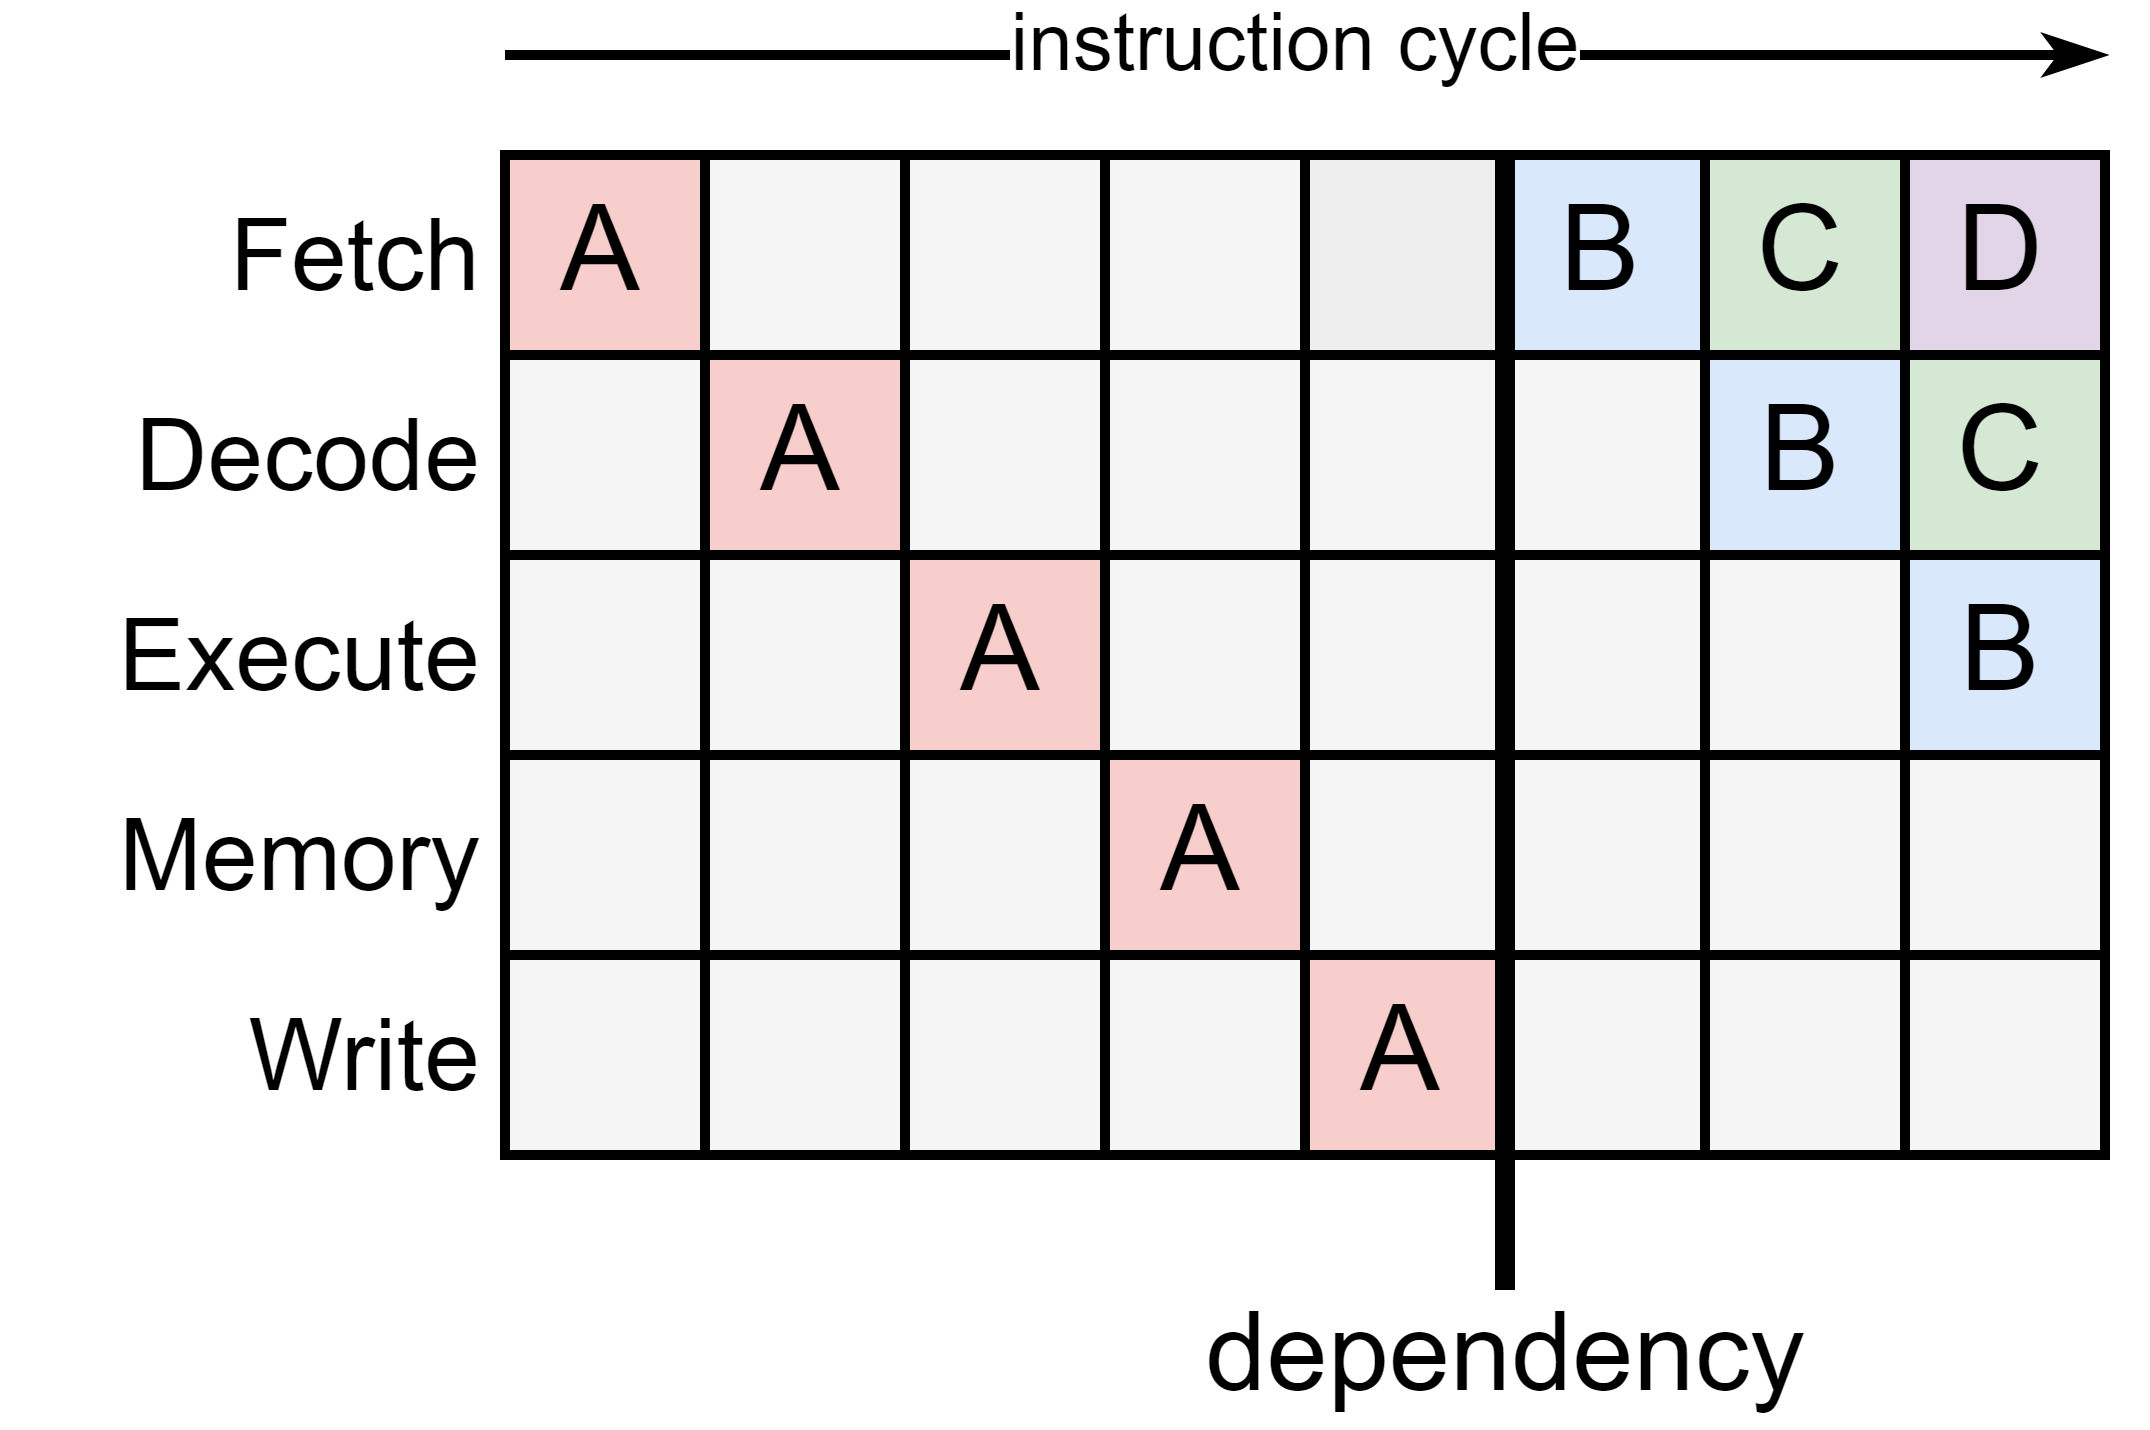
\includegraphics[scale=0.09]{Performance8.png}
        \captionsetup{margin=0.5cm}
        \captionsetup{format=plain}
        \caption
        { 
            Updated instruction-level pipeline where B is dependant on the result of A.
        }
    \end{minipage}
\end{figure}

\vspace{-0.5em}

Specialized processors where an instruction sequence is distributed over many cores are limited to executing all branches unconditionally.
This is minimized through the use of Streaming Multiprocessors (SM), which contain several cores and fetch their own instructions.
Streaming Multiprocessors operate and schedule warps, which often contain 32 threads.
When divergence between these threads occur ({\it branch divergence}) the instructions will in the general case be executed in lockstep\cite{threads-independent-scheduling}.
This means diverging execution flows are not necessarily problematic when it only occurs between different Streaming Multiprocessors, as branches that are not executed can be skipped entirely.

\newpage

\subsection{Data structures} \label{data-structures}

A fundamental aspect of computing is data structures, which is a constant overhead for all computations.
For collective operations arrays are essential; as they have a constant access time, are contiguously allocated and access can be parallelized.
Composite datatypes within arrays introduce some considerations.
One is the {\it implicit} use of parallel arrays, where each primitive datatype is stored in a distinct array.
It enables vectorization opportunities, but a random access pattern might cause additional cache blocks to be cycled between.
Since collective operations control the access pattern, parallel arrays are often a natural choice for array languages.
The consideration for both structurally and functionally distinct data, now referred to as variant, is often complex.
It is at the essence of why non-uniform data demands control over the low-level representation.
Variants can be represented on an individual basis (element-wise) or collectively (variant-wise).
Usage and implementations of these approaches are explored in this chapter. 
Within this chapter the assumption is made that parallel arrays are used, as they align with the intention to vectorize operations. 

\subsubsection{Element-wise}\label{element-wise}

For each individual element the choice of variant is represented, which introduces branching and in the general case will break vectorization.
As variants are not grouped, functions cannot iterate on a specific variant without iterating on the complete array.
The main advantage is that a variant change can be done independently of other elements, and thus can be parallelized.
A practical consideration is that each element in an array must be structurally the same, that is they occupy the same memory space.
This is a limitation which enforces that each index can determine the location of an element. 
For parallel arrays this restriction intuitively applies for all arrays individually\cite{accelerate-sum-types}.

\paragraph{Memory Representation}

Another restriction is that memory instructions only operate on fixed boundaries, which means operations that overlap these boundaries require additional but strictly unnecessary instructions.
A natural alignment of a datatype is achieved by aligning all types according to the instructions that access them.
Many compilers introduce {\it padding} to enforce natural alignment for all the types within the structure.
While computational efficient, the alternative of {\it packing} types together can be preferred for a smaller memory footprint.  

\begin{figure}[ht]
    \subcaptionbox{Compact packed struct of 5 bytes}[.45\linewidth]
    {%
        \centering
        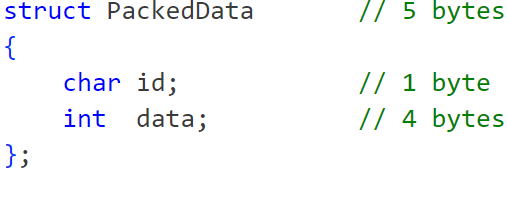
\includegraphics[scale=0.5]{CodeMemory1.png}%
    }%
    \hfill
    \subcaptionbox{Naturally aligned padded struct of 8 bytes}[.45\linewidth]
    {%
        \centering
        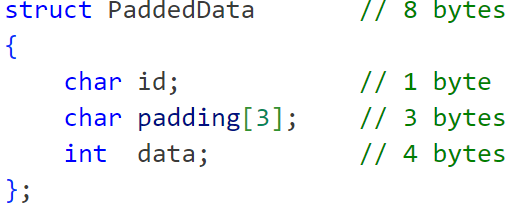
\includegraphics[scale=0.5]{CodeMemory2.png}%
    }
    \caption
    {
        As \type{data} has a size of 4 bytes, padding the \type{id} to 4 bytes enforces that \type{data} is naturally aligned for the instructions that access it.
        In the case \type{data} is stored before \type{id}, the \type{data} type will not always be naturally aligned when stored within an array.   
        It would require padding the complete struct to a multiple of the largest field, which in this case would be 8 bytes regardless.
    }
\end{figure}

Parallel arrays have a natural alignment by default as they only consist of primitives types, which are inherently naturally aligned.
A zero-cost abstraction that can ergonomically switch between Struct-of-Array and Array-of-Struct arrays is non-trivial.
An intermediate structure as interface can break automatic vectorization\cite{abstraction-vectorization}. 
In addition, all the distinct internal representations must be statically definable and able to be handled by the data structures independently.
Many C++ libraries utilize {\it class templates} to achieve this\cite{abstraction-vectorization}.

\paragraph{Tagged Union}

Multiple variants can be represented by a fixed size data component with multiple interpretations, so called {\it union}.
A tag can be used to identify the currently active interpretation of the union. 
A naive implementation creates a new field for all fields within the variants, which means the memory usage is cumulative for each variant within the union. 
A compact tagged union overlaps fields of variants, as only one interpretation can be valid at a time.
The process of overlapping fields is generally referred to as {\it deduplication}.
It can in theory reduce the size to the largest variant within the union, but this is not necessarily computationally efficient due to the previously discussed alignment requirements\cite{accelerate-sum-types}.
A deduplication algorithm for unions therefore balances between enforcing natural alignment and compactness of the memory representation, a space-time tradeoff.
The most primitive form of deduplication is to combine fields that are of the same type.
It can be extended for types of the same size, which would require support for reinterpretation of data.
A consideration for this approach is that it is not apparent how to deduplicate fields of different sizes.
Is it acceptable to pack a byte and short within an integer, or should the individuality of each datatype be preserved.
The individuality of a primitive type is essential for parallel arrays, as it allows for efficient vectorization.

\begin{figure}[ht]
    \centering
    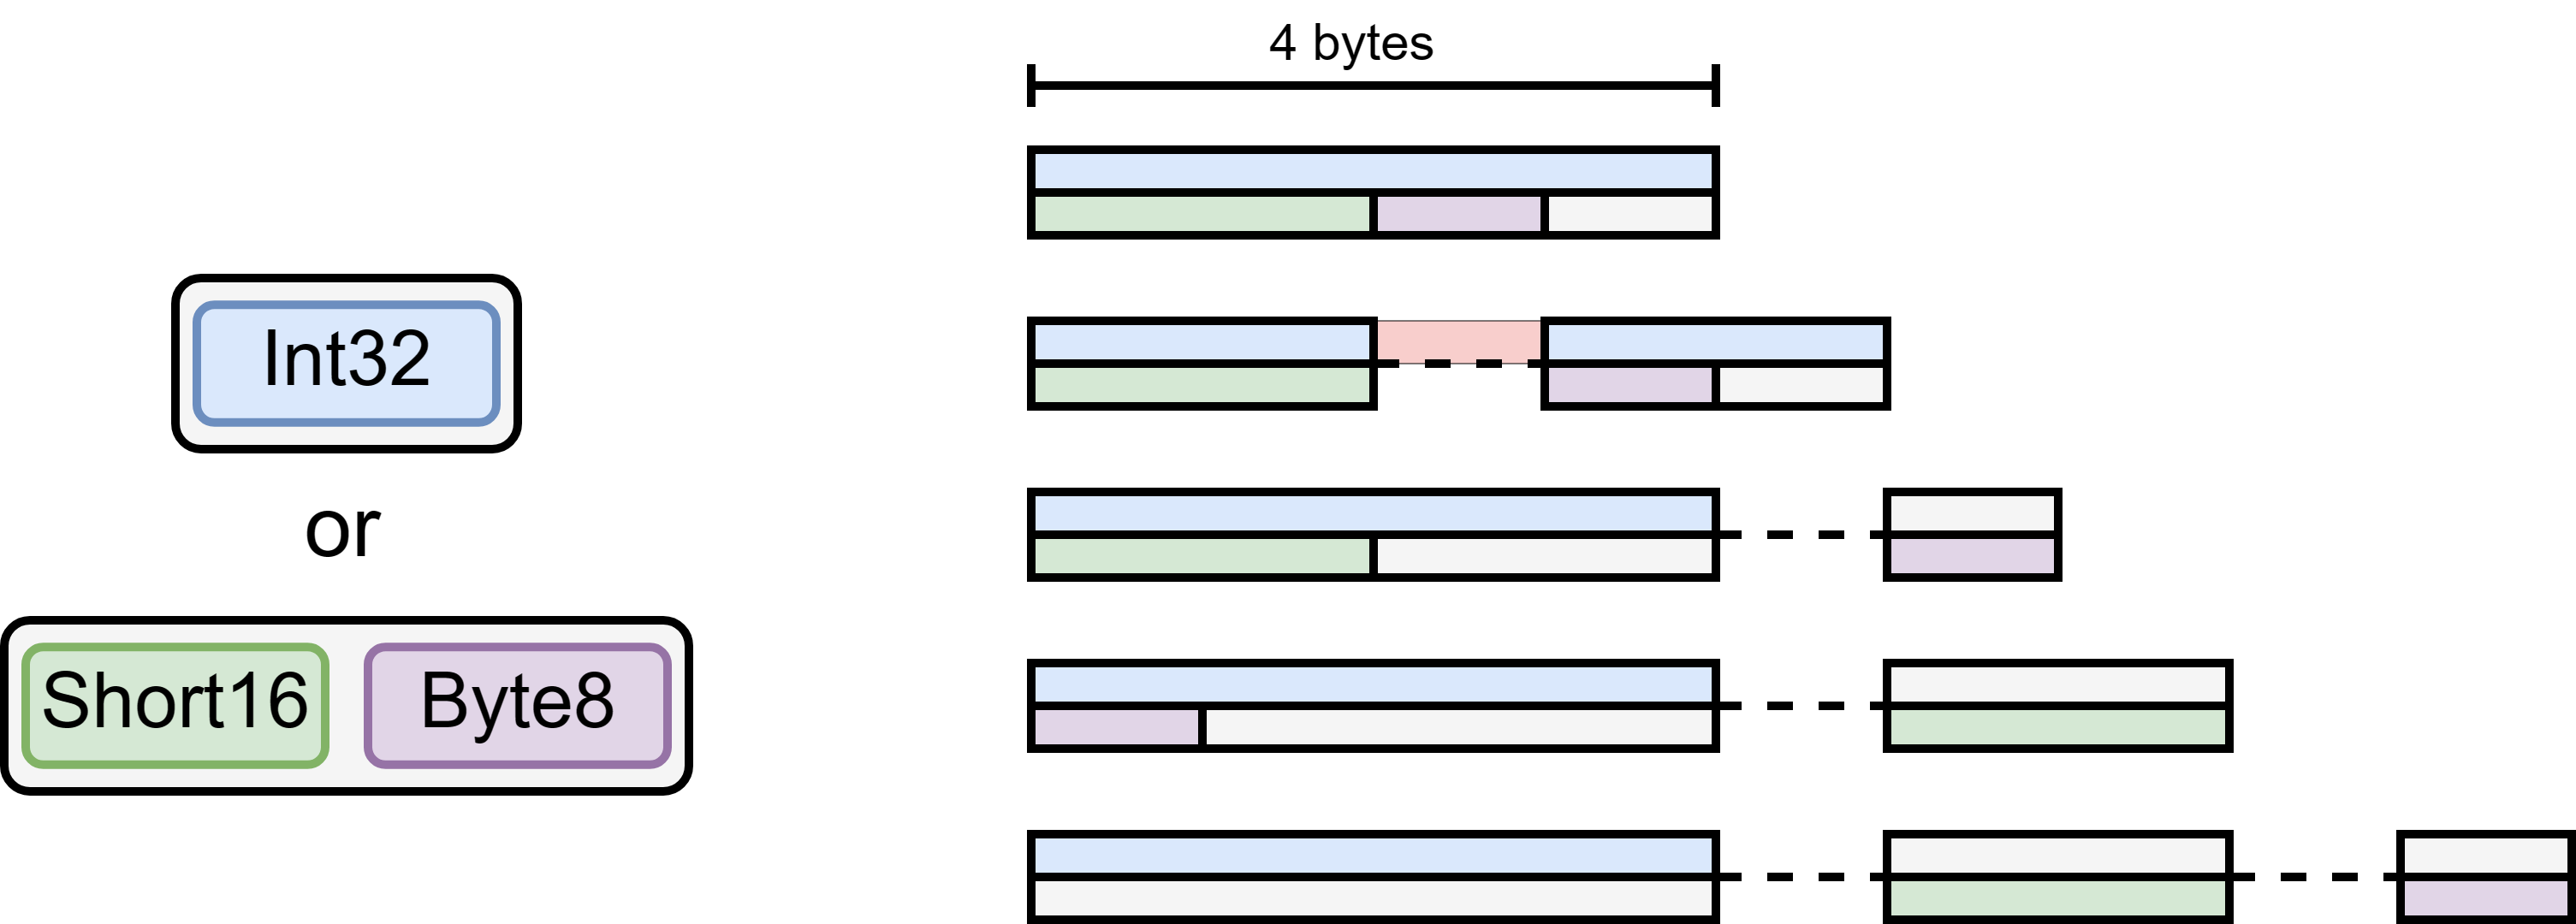
\includegraphics[scale=0.1]{TaggedUnion.png}
    \caption
    { 
        Example of an union type that can either be an integer or a byte and a short.
        The dotted lines within a layout represent a parallel array.
        The first layout is compact, while the other layouts preserve the individuality of at least one primitive type.
        Performance of each layout would depend on which fields are accessed by what instructions.
    }
\end{figure}

General-purpose languages avoid this discussion by overlapping the complete variant, irrespective of the individual fields within the variants.
As stated previously, this would prevent vectorization as fields are no longer contiguous. 
Strictly speaking it can be considered less problematic for tagged unions as there already exists branching on the tag which breaks vectorization, but this does not necessarily always hold.
A form of unconditional execution or compatibility with existing architecture might make a tagged union spread over multiple arrays preferable.
Parallel arrays also make it also possible to enforce natural alignment, as an alternative to padding.

\paragraph{Tagged Pointer}

Another way to comply with elements being structurally the same is to use a form of indirection, in this case a pointer to a memory location.
The indirection allows variants to escape the uniform size restriction, but there are several notable complications.
General complications around pointers, such as being unsafe to operate on and complicating garbage collection apply.
In addition, pointers that point to the same data (alias) can prevent parallelization due to possible race conditions.
These can be partly solved through language constructs; such as smart pointers, immutable data or abstracting the use of pointers altogether.
The key issue is that a change in variant requires new data to be allocated and the pointer to be adjusted.
The allocation means there is no guarantee that the data is contiguous, which in addition to the required branching prevents any vectorization efforts.
The indirection and fragmented memory is also problematic for cache efficiency, as it is unpredictable and a cache block is not used effectively.

\newpage

\paragraph{Entity}

A notable observation is that the re-allocation caused by the variant change causes the data to be not contiguous, not the indirection in itself.
The concept can be illustrated through a hash table data structure, where a key is mapped to a value within an array (bucket).
Any collective operation on the hash table can be vectorized by disregarding the hashing operations and using the internal array directly, as computations are inherently independent and order is irrelevant.   
The indirection is not inherently problematic, merely the use of indirection to denote the identity of an variant.
In essence, a form of indirection that is not used by the collective operations. 
The entity-component-system (ECS) is a coding pattern that sometimes utilizes this concept to efficiently represent collections of multiple variants.
Represented as a single heterogeneous collection, while internally it consists of several variant-wise collections. 

\begin{figure}[ht]
    \centering
    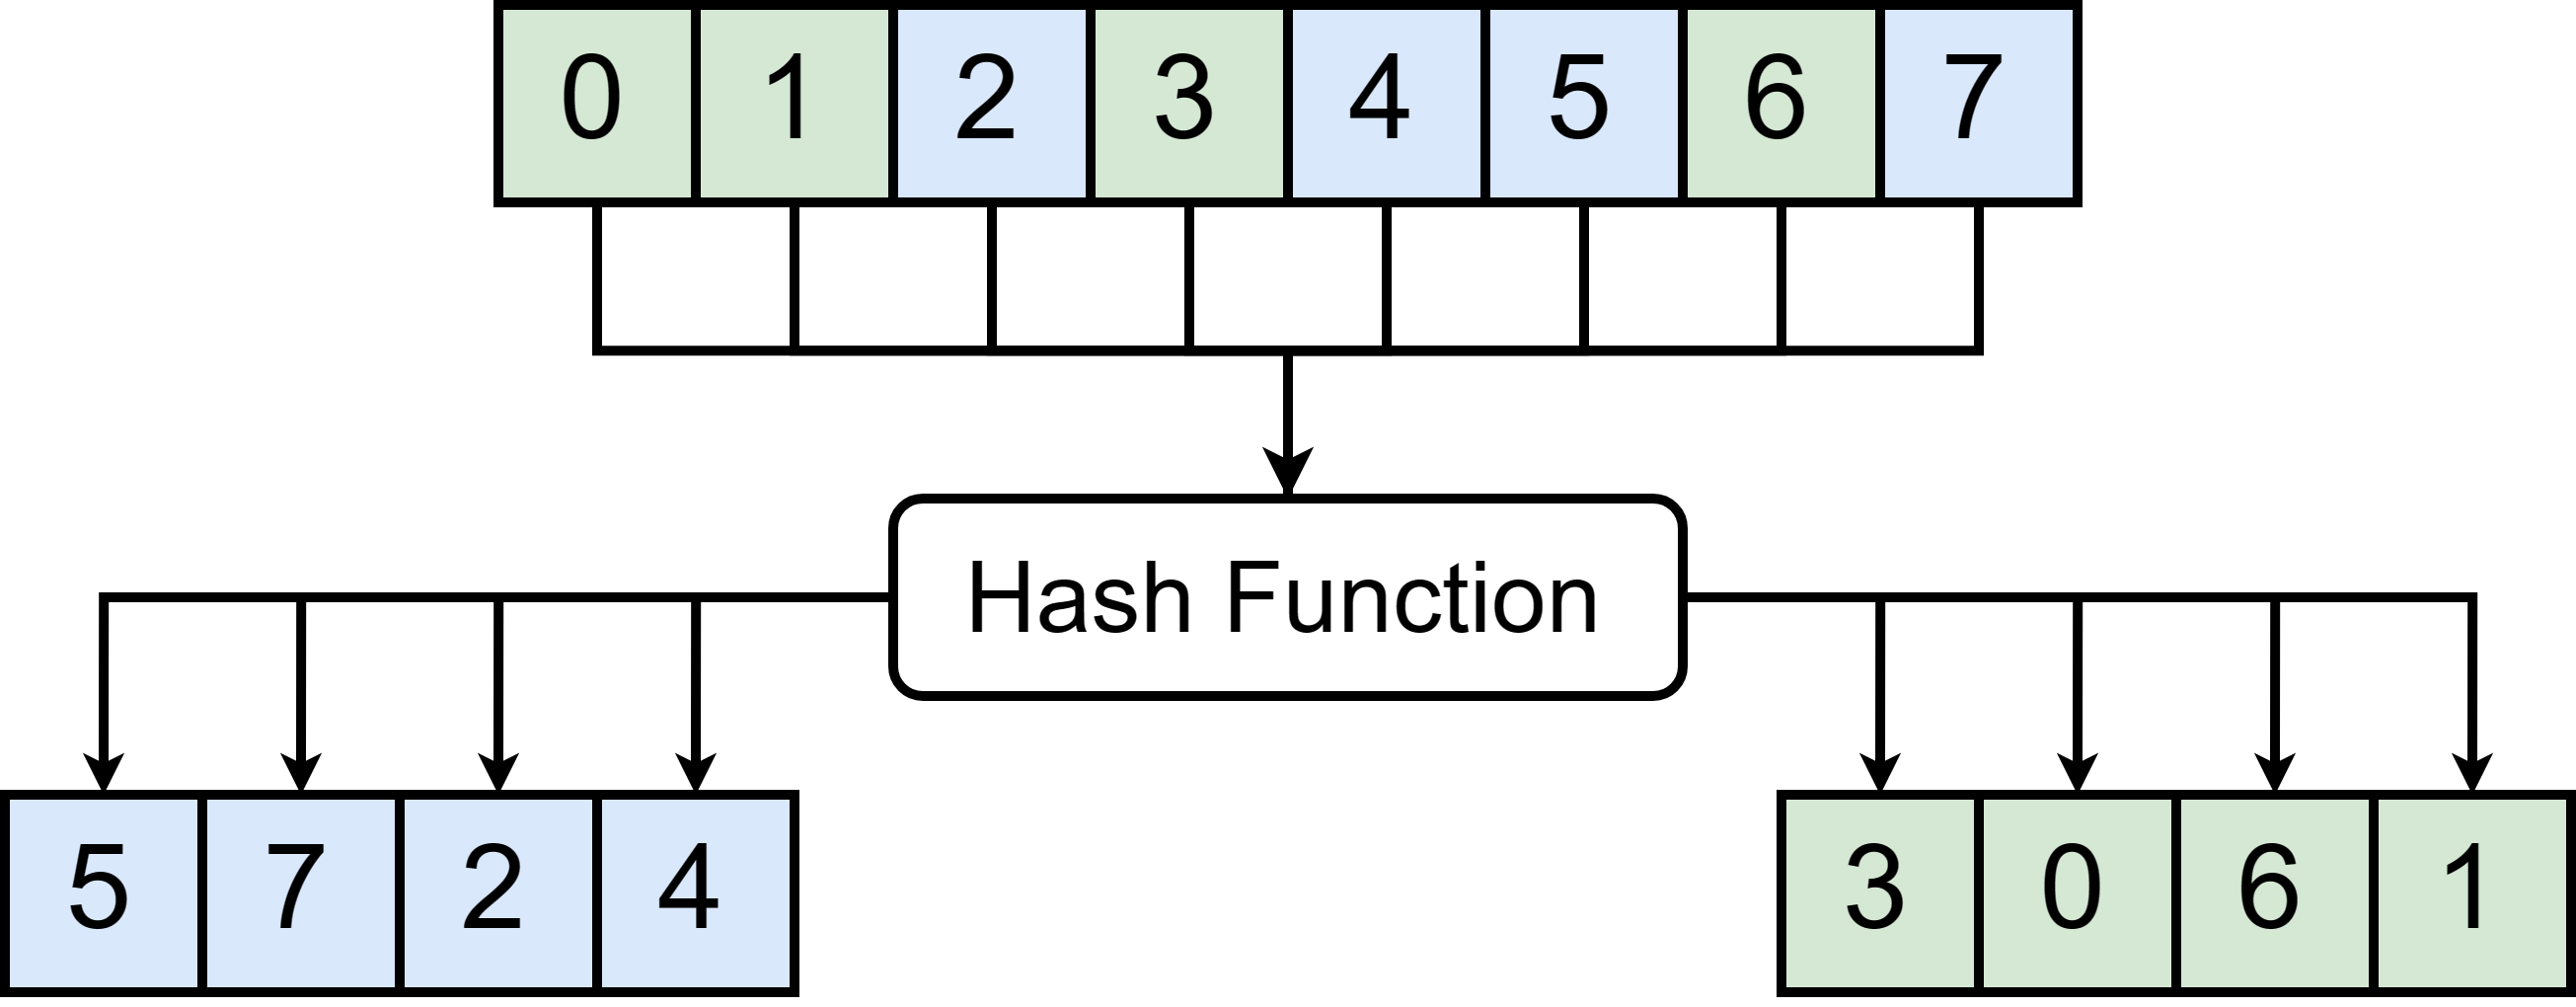
\includegraphics[scale=0.1]{HashTableECS.png}
    \caption
    { 
        Each entry within the surface array can uniquely identify the variant and index through the hashing function.
        The relative costly operating of using the hashing function can generally be avoided, by operating on the variants directly.
        It allows the collection to appear as a heterogenous collection, while still being able to vectorize collective operations.
    }
\end{figure}

It will mean that variant choice is not {\it directly} represented on an element basis, now referred to as an {\it entity}, which has several implications.


\begin{itemize}
    \item [Stable] 
The same entity is not guaranteed to refer to the same data, as the location of the data might change when the variant changes.
The reverse also holds, the data is not guaranteed to have the same entity.
Concretely, the entity is no longer stable across structural changes as it depends on the relative location of the data.
It can solved by maintaining a logbook, by updating the entities with the location of data {\it or} annotating the data with their entity. 
These approaches can be complementary for performance reasons, but they are inverses of each other through gather and scatter operations. 
For many collective array operations stableness is excessive, as it means data is discriminated based on the index of the data. 
    \item [Independent]
Elements can no longer change their variant independently of other elements, which can be problematic when considering data-parallelism.
Depending on the way variants are grouped, there can also be a significant cost associated with regrouping variants.
It can be minimized by delaying structural changes indefinitely, by using the previously discussed tagged union approach.
Regrouping variants can be seen as a performance consideration between the cost of regrouping and having to branch for future iterations.

\end{itemize}    

\newpage

\subsubsection{Variant-wise}

Grouping variants means all data is uniform, contiguously allocated and there exist no inherit branching within the same grouping of variants.
It can be achieved through an array for each variant, but also grouping {\it within} the same array and using segment descriptors.
The latter is effectively an untagged union, where the representation is determined by the index within the array.
Both allow operations to be vectorized, but there exist several other considerations.

\begin{itemize}
    \item [grouping]
    As stated in the previous section, regrouping variants to a variant-wise collection is a performance consideration.
    When variants are stored in separate arrays, the amount of a certain variant must be known before allocation.
    When this is dependant on a computation, it can be retrieved through an additional scan or by atomically\footnote{Atomic instructions prevent interruptions by other processes and are thread-safe.} counting any structural change.
    This adds an overhead, which is not required for a singular array when the total of elements remains the same.

    \item [immutable]
    An important consideration for purely functional languages is that values, and therefore arrays, are to be considered immutable.
    This means that {\it{updating}} parts of an array efficiently is non-trivial.
    It must be proven that the array before update will never be used again, otherwise both arrays must co-exist in memory.
    This is inefficient for small updates and grows the necessity to {\it destructively update}\cite{destructive-update-array}, which is not always possible.

    \item[automatic]
    Most compilers support automatic vectorization of iterations with flexible bounds, where the final leftover iteration is not vectorized.  
    This overhead can be a significant when the loop is extensively unrolled.
    It is minimized through epilogue vectorization, which (re)applies loop vectorization to the remaining scalar code.
    In practice data must be aligned along specific boundaries to be vectorized, which is challenging for dynamic regions within an array and not always analyzed by compilers\cite{automatic-vectorization}.

    \item [operable]
    An undiscussed benefit of parallel arrays is that fields can be operated on independent of other fields, as they are completely distinct arrays.
    This is also possible for {\it regions} within an array, but this is less trivial and often requires explicit support in array languages\cite{accelerate-independent-regions}. 
\end{itemize}

To summarize, there are many variant-wise collections that vary in the organization of the concrete data. 
Either within the same array, spread out over of multiple arrays, or a hybrid which maximizes contiguous memory of only a certain field within the datatype. 
It translates to iterating over a variant-wise collection as well, as one can either iterate over each variant separately (split) or within the same collective function but branch on the index to get the concrete variant (joined).
The split iteration is suitable for vectorization, while the joined iteration reduces potential overhead of having multiple functions and increases the cache predictability.
The concept of a variant-wise collection can be extended further by considering other data structures, which are generally dependant on the specific type of data.
The initial example of an acceleration structure for geometry intersection is such a tailored data structure.
While there are many examples of such data structures, a common pattern for variant types in particular is a shared component.
Rather than organizing based on the variant, it can be beneficial to organize around the types of which the variant is composed.

\newpage

\section{Polymorphic Variants}

A synopsis of the background chapter is that a performant representation cannot be derived from a mere theoretical framework.
There are considerations for both computational efficiency and memory efficiency.
Concretely, an optimal solution is based on factors such as: whether the operations can be vectorized, the required access pattern, if the application is memory-bound or compute-bound, the hardware and the frequency at which the data is used.  
The concept of organizing the program structure around data transformations is referred to as {\it data-oriented design}.
With this in mind it is important for high performance oriented applications to be flexible in the internal representation of their datatypes, as there is not a concrete optimal solution for all situations.
In this case flexibility entails that no architectural changes will be required for changing the internal representation of a datatype.
It is especially important for variant types, due to the previously discussed numerous amount of suitable data structures available for variant types.
In this chapter a solution is discussed which can capture the different data structures in a type preserving manner without sacrificing performance. 
In section \ref{framework} requirements are discussed, with the proposed solution of a type-level variant type.
In section \ref{type-level} and \ref{datatype-generic} we show how type-level programming and datatype-generic programming can be used to implement such a type-level variant type.

\subsection{Requirements}\label{framework}

As discussed in section \ref{data-structures}, there are two primary categorizations for collections of variant types.
Variants of a particular type can be stored either on an element-basis or a variant-basis.
There are several considerations for designing a data structure that is agnostic to whether an element-wise or a variant-wise data structure is used.
A variant-wise collection can operate on a subset of variants, while an element-wise collection is forced to discover the identity while iterating.
To avoid redundant iterations for variant-wise collections, it must be possible to define a function on a specific subset of variants.
For element-wise collections the number of variants must be finite, the type must be identifiable and no large discrepancies should exist between the size of each variant.

\begin{figure}[ht]
    \centering
    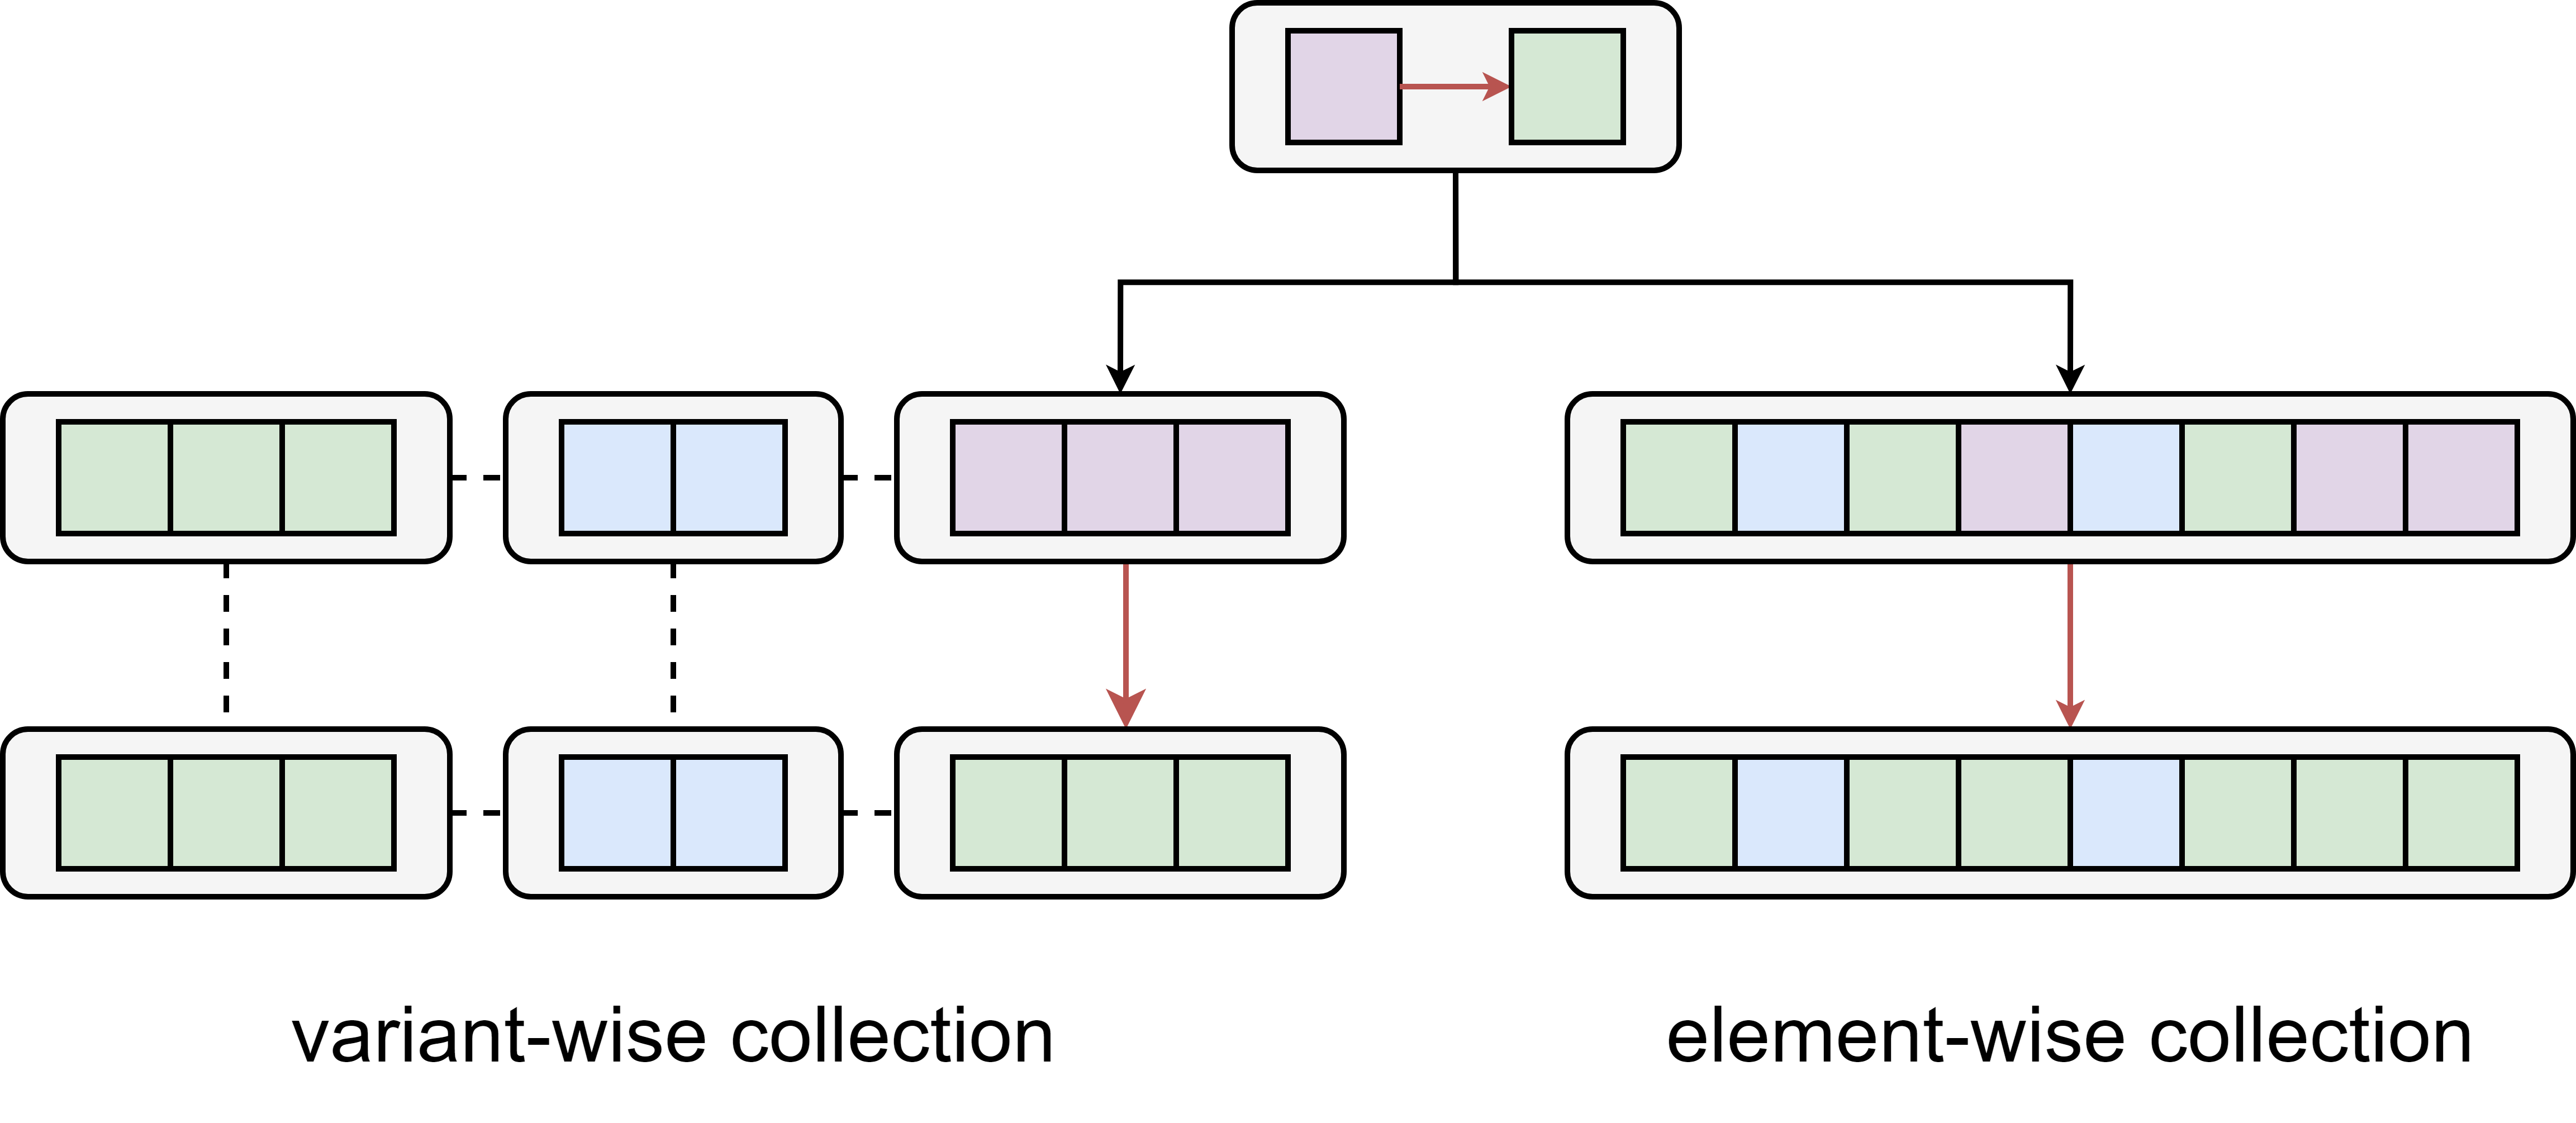
\includegraphics[scale=0.06]{ConceptualFramework.png}
    \caption
    {
        Example where a function is applied on a single variant.
        A non-exhaustive function can skip a significant amount of work when using a variant-wise collection, while this requires a complete traversal for an element-wise collection. 
        Note that the identity of the collection remains the same in both cases (green and blue variant).
    }
\end{figure}

An Entity-Component-System (ECS), previously mentioned in section \ref{related-work} and \ref{element-wise}, allows functions to be defined on a subset of variants.
It is commonly associated with data-oriented design, in particular within the field of game-engines.
Section \ref{ecs} explains the ECS pattern and identifies the core principles around variant-wise collections.
For element-wise collections sum types can be used to safely discriminate between multiple variants by enforcing pattern matching.
Section \ref{adt} is dedicated to sum types and their role in establishing a type-safe interface.  

\newpage

\subsubsection{Entity-Component-System}\label{ecs}

The ECS pattern arguably originated in the context of object-oriented languages being predominant in game engines.
The premise is to organize game-logic around functions, where the relation between data remains flexible\cite{ecs-origin}.
It is in contrast with inheritance, where relations are statically determined.
An overview of the pattern:

\begin{itemize}
    \item [Entity]
    A set of components, where the composition is defined at runtime.
    As such there is no predetermined relation between any of the components.  
    As example, an entity can gain momentum at any time by attaching the \type{Velocity} component.
    \item [Component]
    An user-defined datatype within the pattern, such as \type{Velocity}.
    In the general case components are stored in parallel arrays to exploit data-parallelism opportunities.
    \item [System]
    A global function that repeatedly operates on all entities that match a set of components.
    A \type{Movement} system operates on all entities that contain the \type{Velocity} component, irrespective of other components that might be attached to the entity.
\end{itemize}

The ECS pattern exists on a similar abstraction-level as array languages, through the use of collective operations.
To reiterate on section \ref{element-wise}, an entity is often implemented as a unique identifier.
Rather than using this identifier to find the associated components, collective operations operate directly on the data components.
It allows for a variant-wise collection as internal representation, but with the functionality of a heterogeneous collection.
As such the pattern is often combined with data-oriented design and can be used to implicitly exploit data-parallelism in general purpose languages.


\begin{figure}[ht]
    \centering
    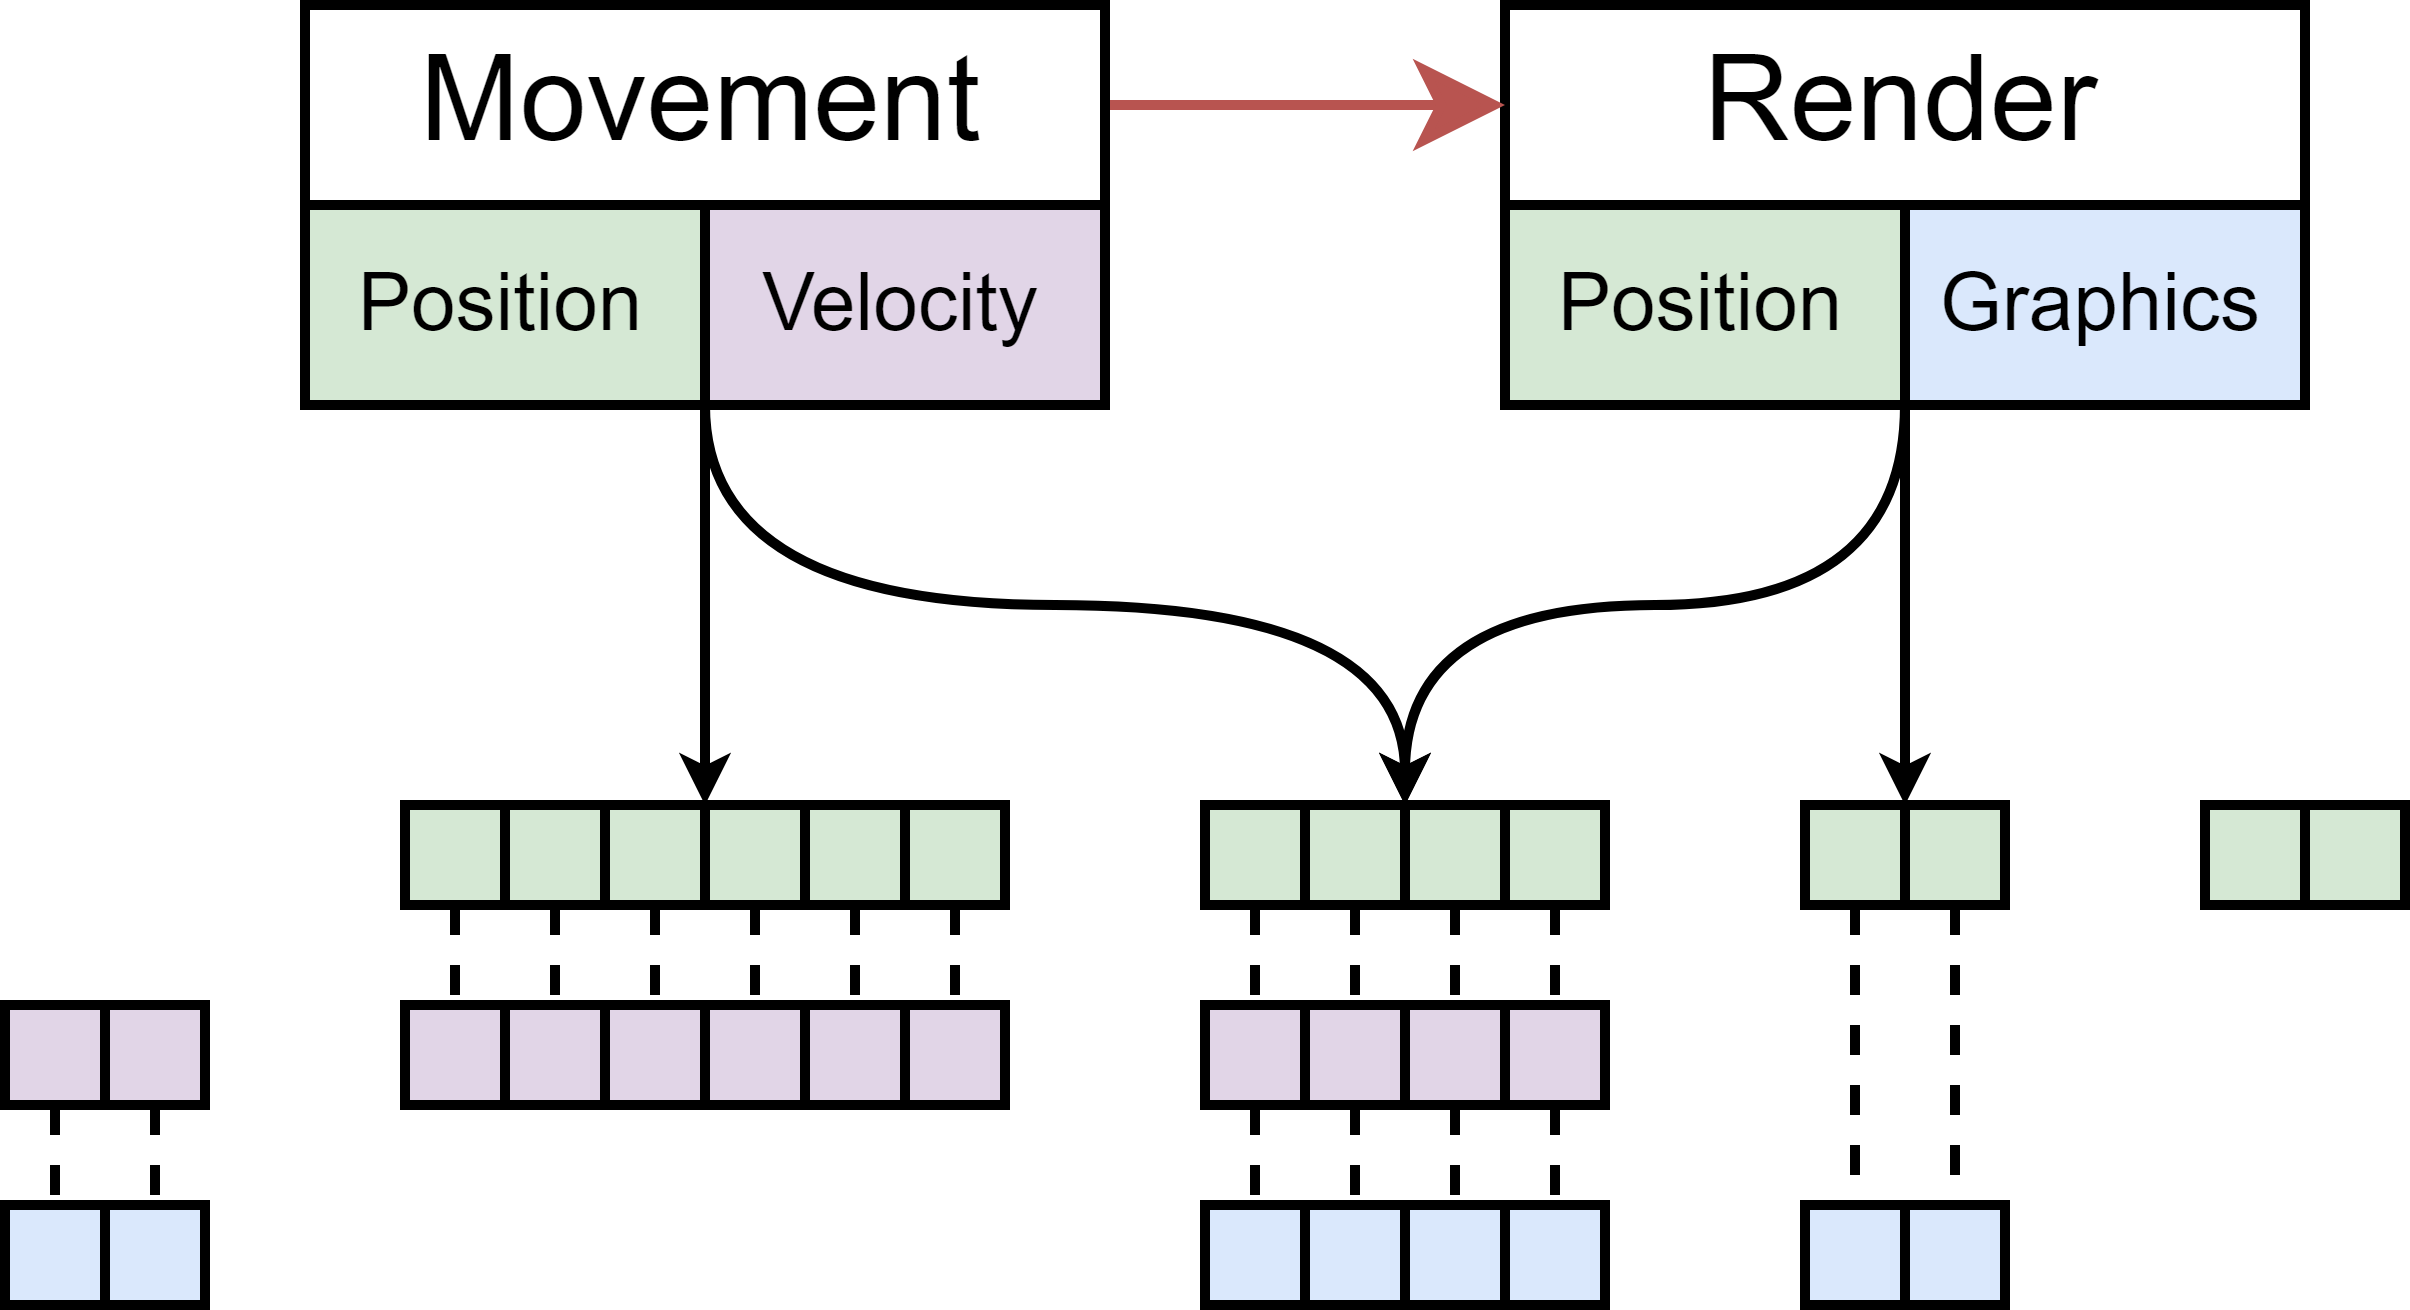
\includegraphics[scale=0.10]{ECSexample.png}
    \caption
    { 
        The movement and render systems both have two components as a dependency and only operate on variants that contain their specific components.
        The example uses a parallel array for each unique combination, so called {\it archetype}.
        Some ECS implementations, such as Bevy\cite{ecs-bevy}, use sparse arrays to speed up the process of adding and removing components at the cost of fragmentation.
    }
\end{figure}


The ECS design pattern is arguably inherently imperative, due the way structural changes are handled.
Apecs, an ECS library in Haskell, achieves this imperative style through monads\cite{ecs-apecs}.
The ECS pattern makes element-wise collections often infeasible, as there is no way to restrict the possible amount of structural changes.
This is inherent to the pattern, as any component can be attached to any entity.
A restrictive approach is to only consider already attached components, by including the ability to {\it disable} a component.
A disabled component is automatically ignored by systems, and is denoted with an element-wise tag.
A more general performant element-wise collection would require a statically definable scope and a notion of mutual exclusivity.
An observation is that the ECS pattern represents variance by the inclusion or omission of a component.
Rather than using the set appearance of entities, we can determine the construct for variant types independently of the performance considerations.
This brings us to {\it Algebraic Data Types}.


\newpage

\subsubsection{Algebraic Data Type}\label{adt}

Functional languages handle tagged unions safely through sum types, which is a construct in an Algebraic Data Type (ADT).
An ADT is a compositional type that categorizes its different compositions with: product, sum and recursive type constructors.

\begin{itemize}
    \item [Product] The composition of datatypes, where datatypes coexist.  
    \item [Sum] The alternation between datatypes, where datatypes are mutually exclusive.
    \item [Recursive] The self referencing datatype, where a datatype is composed of itself.
\end{itemize}

When considering tagged unions, recursive datatypes are infeasible due to their unpredictable and unconstrained size.
This is why only product and sum types are considered.
It is often useful to discriminate between multiple variations of a sum type, which is done through a data constructor.
An example is the \type{Maybe a} type, which represents an optional value. 
It can either be \type{Nothing} or the optional value wrapped in the \type{Just} data constructor.

\begin{figure}[ht]
    \hspace{1em}
    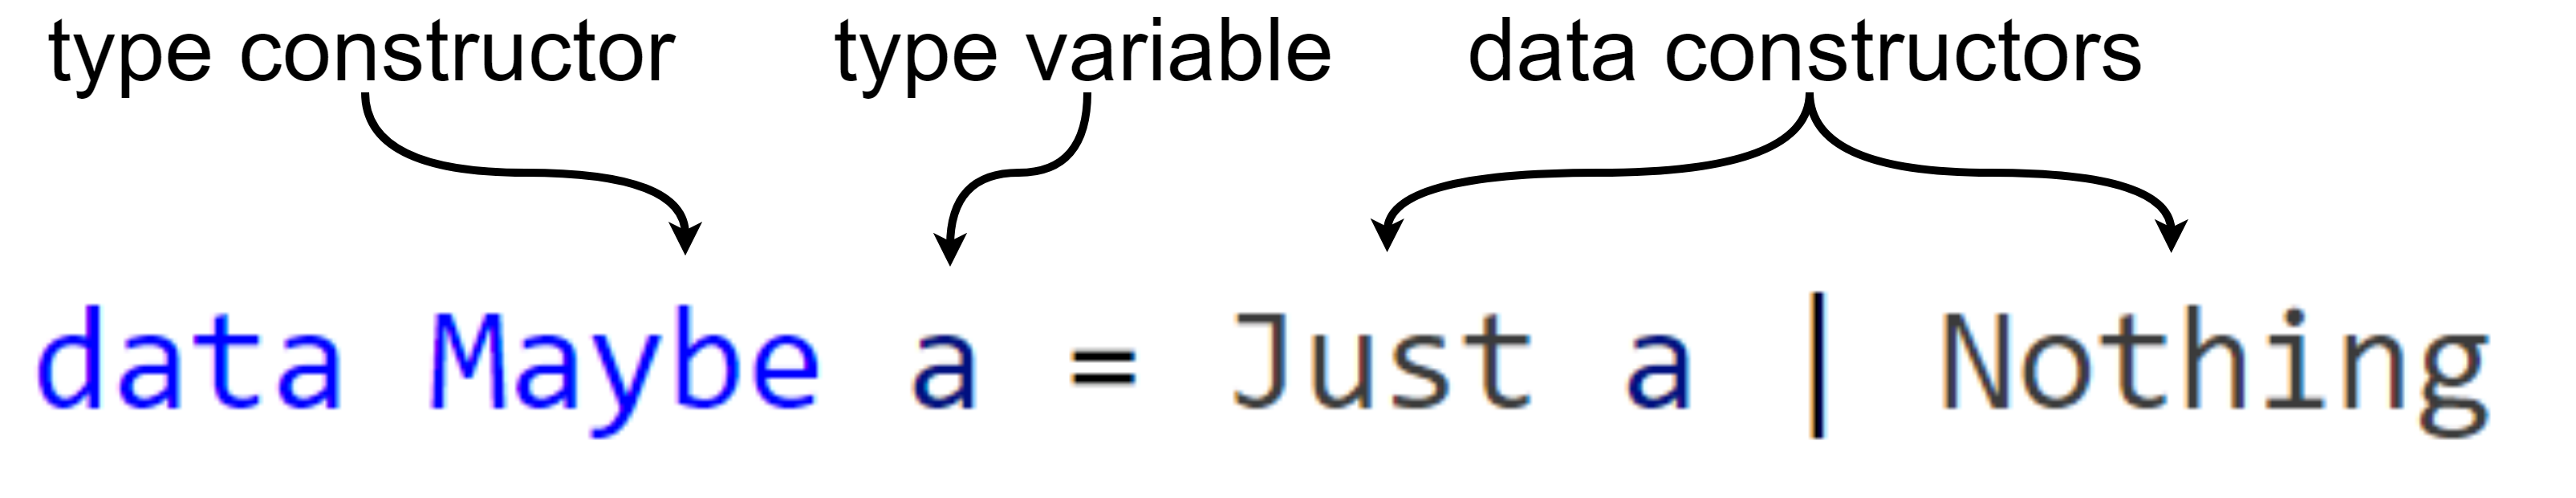
\includegraphics[scale=0.05]{InterfaceCode1Annotated.png}
\end{figure}

Deconstructing an ADT is done by pattern matching on the data constructor.
The pattern matcher can exhaustively match on all variants, as all data constructors are known at compile-time.
It enforces type-safety by ensuring all variants are considered, rather than putting the responsibility on the programmer.
It can be seen as a native control-flow mechanism that ensures only the operations on the active variant are performed.
An example of a function that pattern matches is \type{fmap}, which applies a function to the optional value.

\begin{figure}[ht]
    \hspace{1em}
    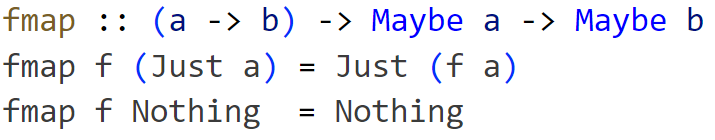
\includegraphics[scale=0.4]{CodeInterface2.png}
    \hypertarget{fig:fmap}{}
\end{figure}

The \type{fmap} function considers two cases, the \type{Just} data constructor and the \type{Nothing} data constructor.
The pattern matcher ensures that the branch of the active variant is chosen, which in the case of \type{Just} would result in the function being applied to the value.
In Haskell, ADTs are distinguishable by name and therefore explicitly declared.
It means data constructors are local to the declared type and pattern matching happens within the same type.
In the context of our intention to create a flexible interface this is problematic for several reasons.
A practical reason is that the ADT must be explicitly declared, which requires meta-programming for a generic implementation.
In addition, on the type-level it is not apparent which variants exist in a particular ADT.
This makes it hard for data structures to adapt to a particular variant type.
It also complicates optimizing variant types that overlap in the variants they contain, as data constructors are local to their type and therefore not necessarily equal.
Consequently, defining a function on a subset of variants is also infeasible.
A solution, which can adapt well to section \ref{ecs}, requires mutually exclusivity to exist on the type-level.

\newpage

\subsubsection{Proposed Solution}

Before discussing the case of sum types, it is easier to start with the case of product types.
A common application of product types are tuples.
The tuple \type{(Bool, Float)} is considered to be equal to any other tuple with the type \type{(Bool, Float)}.
It operates differently from explicitly declared datatypes, which distinguish themselves through their name.
A way to compartmentalize the difference is by considering that a tuple is a polymorphic datatype.
It is therefore also possible to define our own \type{Tuple a b} type, which is only syntactically distinct from a tuple.
A benefit of tuples is that we can define generic functions that take the composition of the tuple in account.
An example is the \type{fst} function, which extracts the first operand of a tuple. 
The concept can be extend to sum types.
In Haskell, the polymorphic \type{Either a b} datatype is either \type{Left a} or \type{Right b}.
The mutual exclusive relationship is captured in a single generic datatype.
Rather than nesting the \type{Either} datatype, ergonomically it is much easier when the arity of the datatype is flexible.
OCaml calls these {\it polymorphic variants}\footnote{OCaml also implements nominally typed sum types, so called {\it variants}.}, while other functional languages generally refer to them as extensible or open sum types.
The operands of the sum type are represented on the type-level, which can be used to solve the previously discussed limitations of nominal sum types in section \ref{adt}.

\paragraph{Motivation}
To make it more concrete, the previously discussed \type{fmap} function is used to demonstrate the flexibility that polymorphic variants provide.
The type signature of the \type{fmap} function provides no information on a potential structural change.
It is possible to return \type{Nothing} for both cases\footnote{\type{Just b} is not possible as it can only be inferred through \type{Just a} and the \type{a -> b} function.}.
From a performance perspective, it means the result of the function will always require a tag.

\begin{figure}[ht]
    \hspace{1em}
    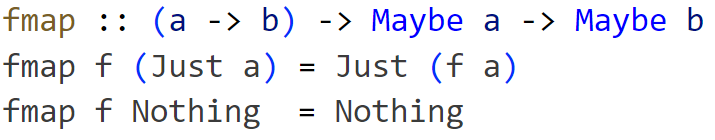
\includegraphics[scale=0.4]{CodeInterface2.png}
    \hypertarget{fig:fmap}{}
\end{figure}


A function that takes \type{Just a} and returns \type{Just b} would ensure that the {\it collective identity} can be preserved.
A variant-wise collection of optional values can therefore prevent the tag and preserve its variant-wise collection.
This exact definition is not possible, as \type{Just a} is a data constructor under the \type{Maybe a} with the type \type{a -> Maybe a}.
As discussed in section \ref{ecs}, it requires a function to be definable on a subset of variants.
In some cases, such as a safe division function, the introduced uncertainty would be inherit to the function.  
The following figure uses the polymorphic variant constructor \type{a || b}, with the standalone \type{Just a} and \type{Nothing} types.

\begin{figure}[ht]
    \hspace{1em}
    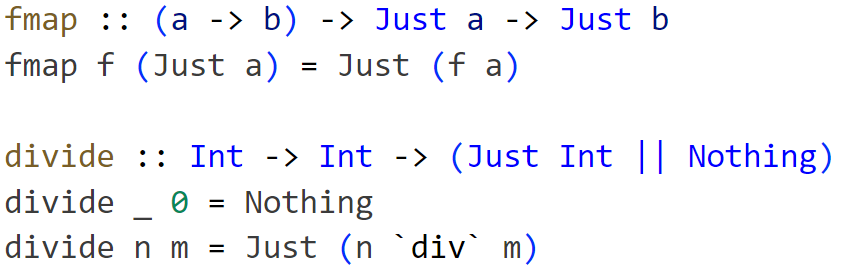
\includegraphics[scale=0.4]{CodeInterface3.png}
\end{figure}

Concretely, \type{Maybe a} is now an alias for the mutually exclusive relationship between \type{Just a} or \type{Nothing}.
A motivating example is that a collection of \type{Maybe a} can now be an element-wise collection or two variant-wise collections of \type{Just a} and \type{Nothing}\footnote{As \type{Nothing} does not hold data, a size descriptor is sufficient.}.
While the former involves branching for \type{fmap}, the latter can ignore the \type{Nothing} collection and vectorize the \type{fmap} function.
An implementation of polymorphic variants will be discussed in the upcoming sections.

\newpage

\subsection{Type-level programming}\label{type-level}

In the previous section polymorphic variants are proposed, a type constructor which represents multiple variants.
It is analogous to a nested \type{Either a b} datatype, but functionally similar to a flattened sum type with data constructors.
Defining an internal representation for each use of a polymorphic variant is infeasible and defeats the purpose of being able to ergonomically switch between representations.
Statically deriving an internal representation for a datatype is impossible in most languages.
Some high-performance libraries circumvent this restriction by meta-programming or having predetermined custom data layouts\cite{llama}.
A type-safe solution is type-level programming, which will be utilized within this chapter to generically derive efficient memory representations.

\subsubsection{Kinds}\label{kinds}

A value is categorized by types, while a type is categorized by {\it kinds}.
This is relevant when discussing type constructors, where type constructors with a different arity have a distinguishable kind.
A well known exposition of type constructors are parametric polymorphic data types.
While a lot of languages support polymorphic data types, the concept of kinds is not evident as only concrete types are used as argument.
Haskell supports higher-order types, which function similarly to higher-order functions, which makes kinds more apparent to the user.

\vspace{-0.2em}
\begin{figure}[ht]
    \hspace{1em}
    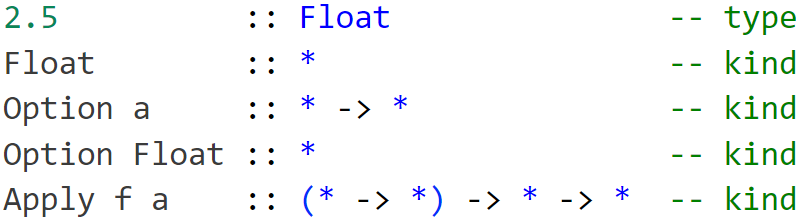
\includegraphics[scale=0.38]{CodeType1.png}
\end{figure}
\vspace{-0.2em}

Type constructors can be used to encode data statically, such as Peano numbers.
The parametric \type{Succ a} and \type{Nil} types are axioms that can be used to construct a natural number on the type-level.
By default these exist in a open universe, which means ill-formed expressions can be created.
On the type-level it can be resolved by Generalized Algebraic Data Types (GADTs), implemented in Haskell as an extension.
The type variables of data constructors can diverge from the more general type.

\vspace{-0.2em}
\begin{figure}[ht]
    \hspace{1em}
    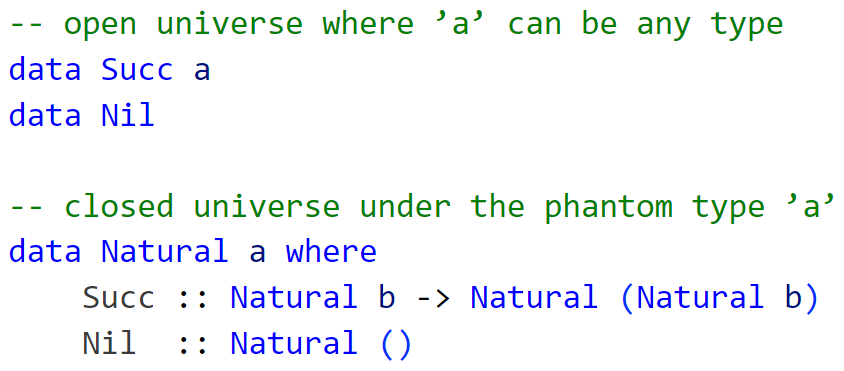
\includegraphics[scale=0.38]{CodeType2.png}
\end{figure}
\vspace{-0.2em}

The consequence is that deconstructing a GADT will refine the type.
Pattern matching can therefore construct evidence of certain properties.
An observation is that this is a categorization of types, similar to how the kind \type{*} represents all concrete types.
The \type{DataKind} extension promotes types to the kind-level and constructors to the type-level. 
The \type{Natural} kind would include the type \type{Succ (a :: Natural)} and \type{Nil}.
It is a kind-level solution, which creates a closed universe and other type constructors can now also use the \type{Natural} kind.
A limitation is that the construction of the kind, which is needed for arithmetic operations, is guarded by the definition of \type{Natural}.

\begin{figure}[ht]
    \hspace{1em}
    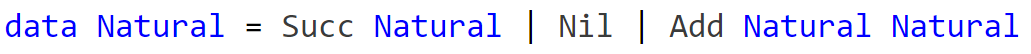
\includegraphics[scale=0.38]{CodeType3.png}
\end{figure}

On the type-level this is solved through value-level functions.
Translated to the kind-level it means we need type-level functions that transform an input kind into an output kind.

\newpage

\subsubsection{Type Family}

A way to approach type-level functions is to see it as a type dependent on the instantiation of a type variable.
This is akin to functions in type classes, where type-indexing allows functions to be overloaded.
Haskell reuses this functionality for types, categorizable as {\it associated types}\cite{associated-types}.
It is particularly useful for embedded domain-specific languages, as an instance can have a specialized return type.
Accelerate uses the \type{Elt}\footnote{Extract, Load, Transform.} class to create a mapping between surface and embedded types.

\begin{figure}[ht]
    \hspace{1em}
    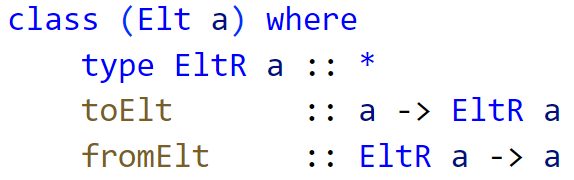
\includegraphics[scale=0.38]{CodeType4.png}
\end{figure}

While these type-indexed types integrate well with type classes, type families is the much stronger standalone concept.
A \type{data family} has unique types associated with each type, while a \type{type family} is merely the type synonym equivalent.
In some cases a function cannot be represented, as the type checker is unsure which instance within the type family to use.
This is the case when the function has a more general default case that will always match.
A closed type family attempts the instances in order of definition, which expresses itself in being able to pattern match on types.

\begin{figure}[ht]
    \hspace{1em}
    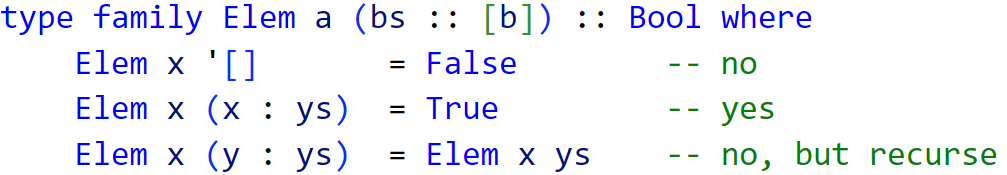
\includegraphics[scale=0.38]{CodeType5.png}
\end{figure}

In this example the variable \type{y} can be \type{x}, which means the second and third instance are overlapping with each other.
A closed type-family resolves this by attempting the more specific case of \type{x = x} first.
A lot of functions can now directly be translated into a type-level equivalent.
An annoying limitation in Haskell is that type families cannot be partially applied, which means a lot of boilerplate is required to capture more complex functions.
Type families cannot be partially applied due to it requiring higher-order unification, which is currently not supported in Haskell.

\subsubsection{Interface}

With type-level functions a type can be computed based on an argument type, which is the foundation for constructing multiple representations for a single variant type.
The process of constructing multiple representations can be captured within a single datatype.

\vspace{-0.5em}
\begin{figure}[ht]
    \hspace{1em}
    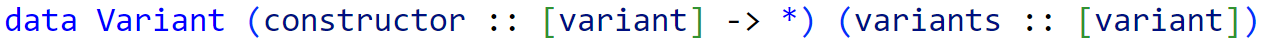
\includegraphics[scale=0.38]{CodeType6.png}
\end{figure}
\vspace{-0.5em}

The data type \type{Variant} takes two type variables, a higher-kinded construction type and a promoted list type.
The constructor takes the promoted list and transforms it into a concrete type.
As type families cannot be partially applied, a data family is used to create the concrete constructor.

\begin{figure}[hbt!]
    \hspace{1em}
    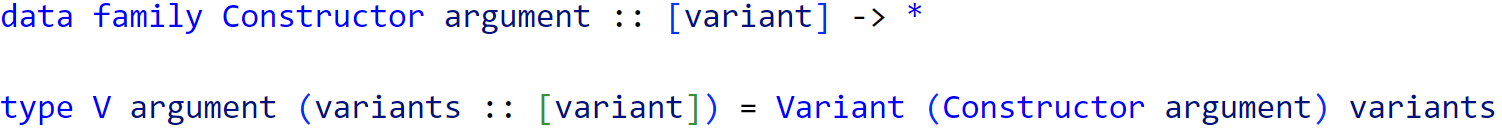
\includegraphics[scale=0.38]{CodeType7.png}
\end{figure}

An instance of the constructor data family constructs a unique type, which is based on the given argument.
It avoids partial application by effectively using the \type{Constructor} data family as a dictionary.
An example variant type would be \type{V Compact [Int, Float, Bool]}, where \type{Compact} is the argument.
The \type{Constructor} data family then constructs the actual type with the kind \type{[variant] -> *}.
 
\newpage

\subsubsection{Type Composition}\label{type-composition}

While it is now possible to abstract over the multiple constructors, the next step is to implement the constructor type.
As a memory representation only concerns itself with the bit size of types, the intermediate structure will be the natural number discussed in subsection \ref{kinds}.
The \type{DataKinds} extension natively supports the \type{Nat} kind with arithmetic expressions and literals for syntax.
While mapping primitive types to their corresponding natural number is trivial, this is not the case for user-defined datatypes.

\begin{figure}[hbt!]
    \hspace{1em}
    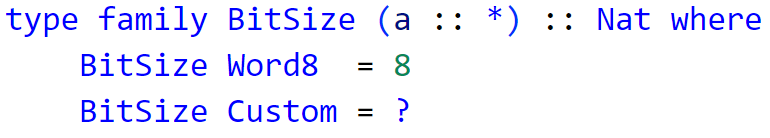
\includegraphics[scale=0.38]{CodeType8.png}
\end{figure}

It is not possible to statically derive the bit size of the \type{Custom} type within the type family.
For this the types of which \type{Custom} is composed of, or the structure of the type itself, must be apparent to the type family.
A way to approach this is to use a kind more specific then \type{*} that is also explicit in the composition, such as the \type{Natural} kind but for all datatypes.
While the approach works on paper, it would involve drastic changes to an existing architecture.
Another way is to enforce an implicit constraint by ensuring the type can be constructed with a particular GADT.
The latter is used by Accelerate, where the \type{TupR} constructor ensures that the embedded type is composed of only primitives types and tuples.
The function \type{eltR} enforces this by requiring the associated type \type{EltR a} to have a mapping to the \type{TupR} type\footnote{Note this can be circumvented by returning a bottom type such as \type{undefined}, which will only be detected when using the value. }. 
The GADT approach is preferable when access to the structure on the value-level is also needed, which is the case for future datatype-generic programming endeavors.

\begin{figure}[hbt!]
    \hspace{1em}
    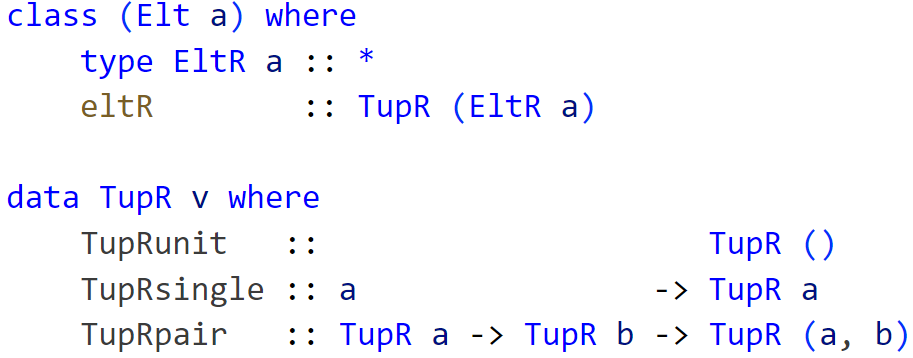
\includegraphics[scale=0.38]{CodeType9.png}
\end{figure}

With this constraint it is now possible to figure out the bit size of user-defined datatypes.
A closed type family is used to recursively traverse the structure, where primitive types are converted to their respective bit size.
It lays the foundation for type-level programming on user-defined datatypes.

\begin{figure}[hbt!]
    \hspace{1em}
    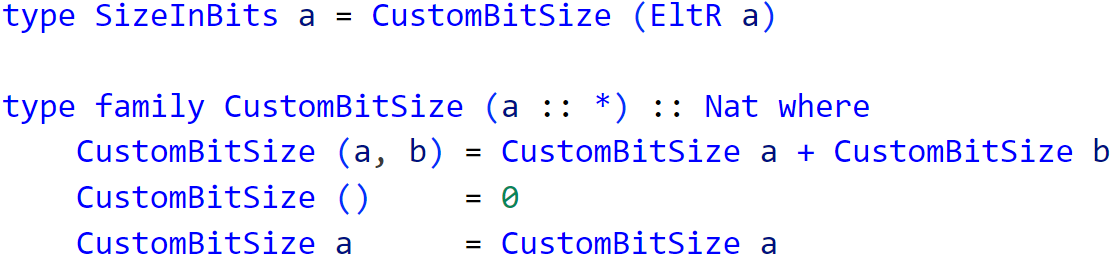
\includegraphics[scale=0.38]{CodeType10.png}
\end{figure}

In Accelerate the embedded representation is the one relevant for optimizations.
All type-functions therefore operate on the embedded representation, the type associated with \type{EltR}.
It is impossible to construct such type outside the \type{Elt} class.
A solution is to automatically derive the \type{EltR} class for a set of types with a fixed representation, such as tuples. 
Returning a type with a fixed representation means that all computed representations will inherently implement the \type{Elt} class. 

\newpage

\subsubsection{Deduplication}

While the tools are there to generically compute different memory representations, it is not trivial to create a single performant solution.
Capturing all possible solutions to a performant memory representation is made easier by creating an intermediate structure that only contains the relevant information. 
The most general intermediate structure of a composite datatype is a collection where each field in the datatype is represented as their size in bits.
It removes both hierarchy and type identity, which makes it is easier to reason about a specific layout of a datatype.
The intermediate representation will preserve performance critical information about the way data can be retrieved by instructions.
The conversion is analogous to the \type{CustomBitSize} type family, but the the promoted list type \type{[]} is used instead.

\begin{figure}[hbt!]
    \hspace{1em}
    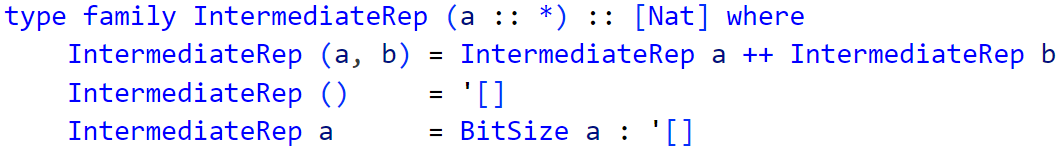
\includegraphics[scale=0.42]{CodeType11.png}
\end{figure}

With closed type-families it is possible to define most of the common operations on lists.
The definition of these are similar to their value-level counterparts, but without any partial application.
As such it possible to define a type-level function that creates a compact deduplicated union.
As stated, the \type{IntermediateRep} function returns a list of natural numbers.
The \type{Union} function recursively adds an element only if it is unique.
The corresponding element is removed from the comparison list once it has been matched.
This ensures all fields of a datatype are included exactly once. 

\begin{figure}[hbt!]
    \hspace{1em}
    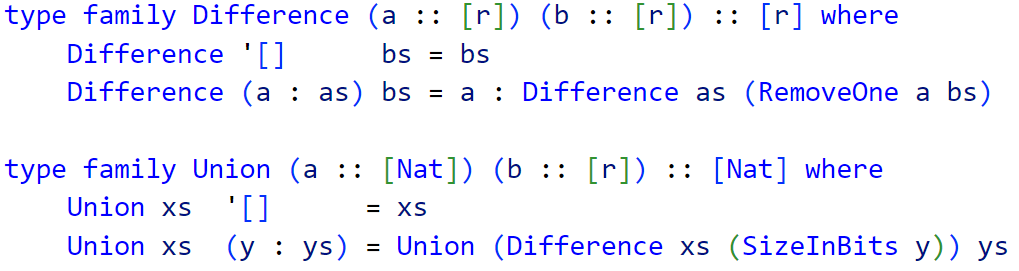
\includegraphics[scale=0.42]{CodeType12.png}
\end{figure}

One could consider the representation compact, but it deduplicates only the bit size of the primitive type that is of equal size.
This is very safe, as there is no inherit performance cost to operating on types with the same size.
This is not necessarily the case for types stored in a larger type, or even a type spread out over multiple types.
In some memory-bound cases this approach can still be preferable.
An implementation would require type-level sorting, to avoid a scenario where the smallest type is inserted into the largest type.
A naive sorting algorithm is quite trivial to implement, by inserting all elements into their respective position. 

\begin{figure}[hbt!]
    \hspace{1em}
    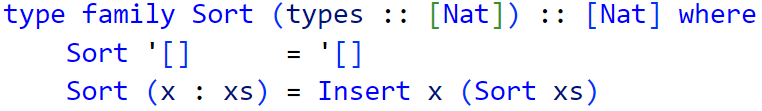
\includegraphics[scale=0.42]{CodeType13.png}
\end{figure}

The derivation of such a compact layout is not particularly complex, as it is similar to the normal deduplication approach but with multiple stages.
Each step increasing the perceived performance cost of the deduplication and avoiding a local optimum solution by unifying large datatypes first. 
The complexities of such layout lay within generically operating on it.
The simplicity is only the case due to implicitly using parallel arrays, as it avoids having to incorporate padding.
When padding is handled the approach can be extended to non-variant types as well, as it effectively is the simpler case of a variant type with only one variant.
To summarize, we can now switch between multiple memory representations for a variant type through type-level programming.

\newpage

\subsection{Datatype-Generic programming}\label{datatype-generic}

In the previous chapter a way was established to compute a wide-range of internal representations for a variant type.
It is not ergonomically viable to write (de)construction functions for all the different representations. 
As users can create their own representations there is no closed system, so mapping between all possible datatypes must be handled.
This can be achieved with datatype-generic programming, which parametrizes on the composition of a datatype\cite{datatype-generic-programming}. 
A mapping must be isomorphic, such that all information is preserved between construction and deconstruction of the union.
This is not possible for all possible pairings, as the variant must be smaller or equal in comparison to the union.
Within the first section a type-level way to prove valid pairings is explored, which is essential for supporting user-defined datatypes.
The second section explores the foundations of datatype-generic programming, which is used for an implementation of a datatype-generic framework in the third section.

\subsubsection{Verifying}

A variant must be smaller or equal to the union it exists in.
A variant that is larger than its union loses information when constructing and deconstructing.
While it is possible to ensure that the type-level computation of the representation is always larger than the variant, this is a risky construction.
It limits users extensibility and does not catch flaws within existing derived memory representations. 
A modular implementation requires an independent method that ensures the variant is smaller than its representation.
The \type{Constraint} kind can be used to restrict the construction to larger or equal types.
Constraints occur on the left-hand side of the type annotation, and are generally used to enforce that an interface has been implemented.
A relevant example is ensuring that our newly computed representation has a mapping to the embedded representation.

\begin{figure}[hbt!]
    \hspace{1em}
    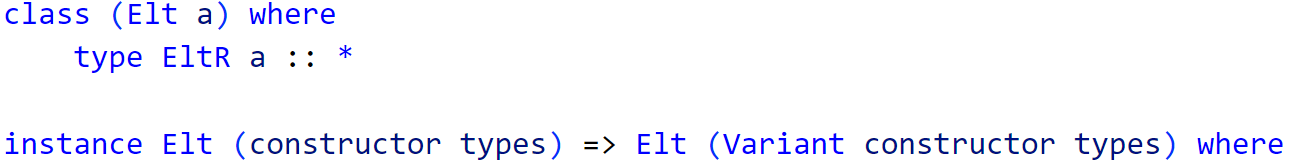
\includegraphics[scale=0.4]{CodeType14.png}
\end{figure}


In the type-level programming chapter we already achieved a way to determine the size of any type, as a \type{Nat} kind.
Fortunately the native \type{Nat} type already supports several comparison operators with the kind \type{Nat -> Nat -> Constraint}.
A simple but functional constraint is the \type{<=} operator.
While it does omit performance considerations, a lax restriction is required to support a wide-range of representations.
A generic class can be used to capture the relation between variant and union nicely, the \type{IsVariant} class.
Operations that require type-safety can use this class, while the general variant type can remain constraint-free with the assumption that the union will be larger than the variant.
The \type{IsVariant} class has a default implementation for constructing and deconstructing, but can be extended by the user to support unsafe variants such as sentinel values.

\begin{figure}[hbt!]
    \hspace{1em}
    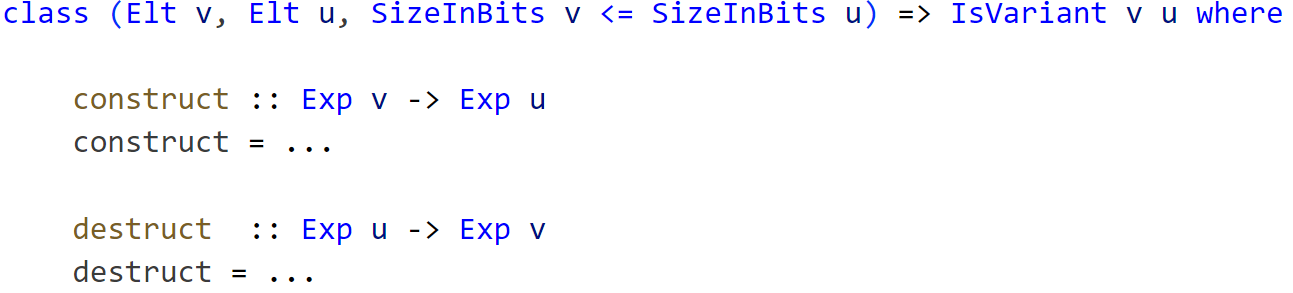
\includegraphics[scale=0.4]{CodeType15.png}
\end{figure}

The \type{IsVariant} class can be restricted further by constraining the individual fields within the datatype.
The next data-type generic programming part pertains to implementing the default \type{construct} and \type{destruct} functions.

\newpage

\subsubsection{Theory}

Before looking into how \type{construct} and \type{destruct} are implemented concretely, it is essential to understand the problem datatype-generic programming is attempting to solve. 
Paradoxically variant types are best to illustrate the problem, coined the {\it expression problem}\cite{expression-problem}.
Extending the variants within the \type{Color} type means all functions that pattern match on \type{Color} must be changed. 
It can be resolved by having a general interface, but extending the behavior of this interface requires all types that implement the interface to change. 
There is no way to extend functionality without having to explicitly define some sort of behavior.

\begin{figure}[ht]
    \centering
    \begin{minipage}{.5\textwidth}
        \hspace{1em}
        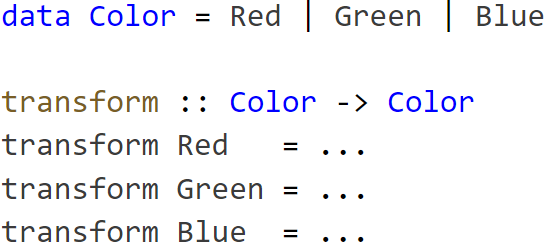
\includegraphics[scale=0.4]{CodeType16.png}
    \end{minipage}%
    \begin{minipage}{.5\textwidth}
        \hspace{1em}
        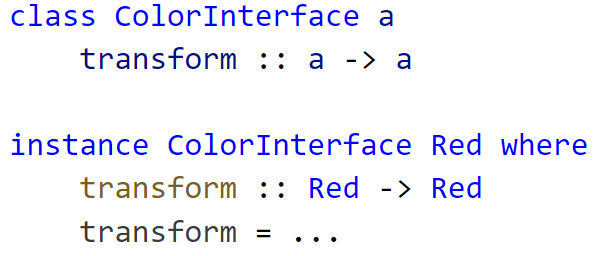
\includegraphics[scale=0.4]{CodeType17.png}
    \end{minipage}
\end{figure}

The impact of the {\it expression problem} can be minimized through several methods. 
Arguably polymorphic variants fit within this category themselves, as it separates pattern matching with the underlying data\cite{polymorphic-variants-expression-problem}.
In our case we have chosen for the representations to be extensible, which requires behavior to be defined for all possible representations.
Both for constructing and deconstructing the union into a specific variant.
The possible datatypes is an infinite domain, which can be made finite by considering that all composite types can always be reduced to primitive types.
Datatype-generic programming utilizes the concept of composition in programming languages to operate on any type.
This is sufficient to generically operate on multiple representations, as the semantics of the type are irrelevant for constructing and deconstructing the variant type.
It requires access to the way type are composed, which is not always natively supported in programming languages.
While Haskell does support datatype-generic programming, we do not operate directly on native Haskell types.
An implementation through native Haskell types, which Accelerate currently uses for sum types, is restrictive.

\begin{figure}[ht]
    \centering
    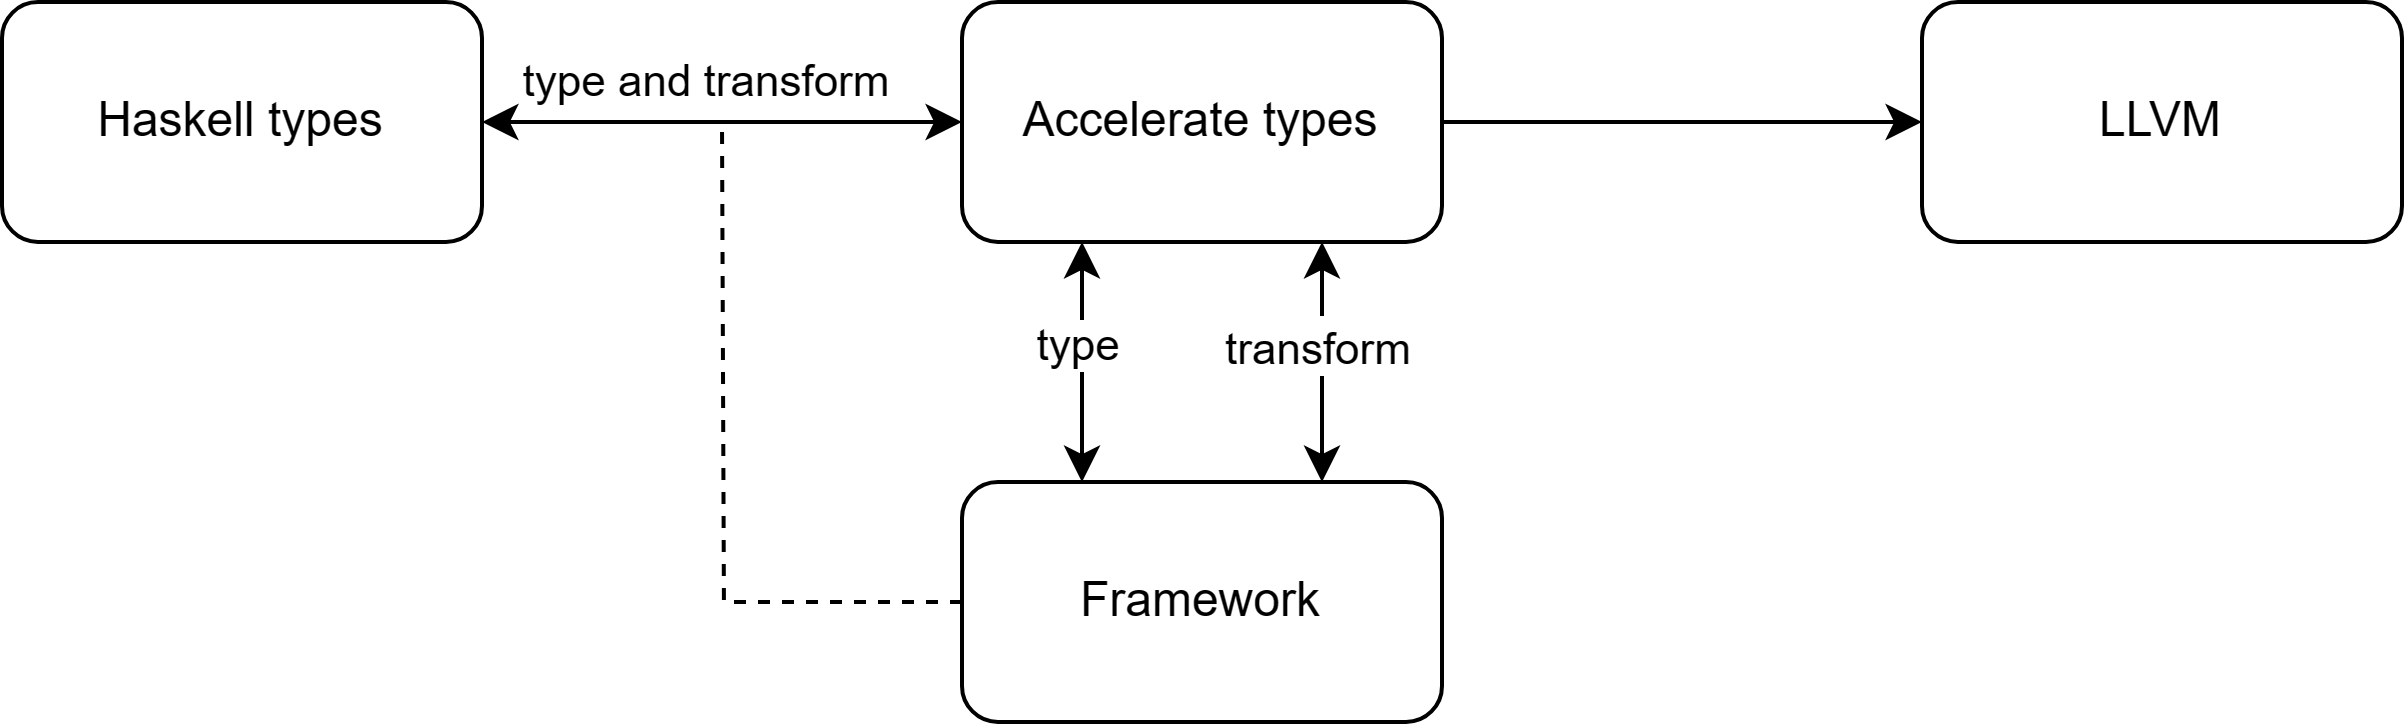
\includegraphics[scale=0.15]{framework.png}
    \caption
    {
        Visual diagram that displays the interconnectivity of data types within Accelerate and the relative placement of the framework.
        Note that the type and transform are separate, which adds to the modularity of the approach. 
        It can be used to implement the translation layer between surface and embedded representations.
    }
\end{figure}

The restrictions are apparent when attempting to implement structurally typed sum types or more complex representations generically\cite{accelerate-sum-types}.
The complexity is caused due to the \type{Elt} class requiring a direct mapping to the Haskell equivalent. 
Each deduplication decision must also be represented on both the value-level and type-level, rather than just the type-level.
The translation layer remains essential for embedded languages, but can be implemented with the help of a standalone implementation.
Operating directly on embedded types results in a more targeted and adaptable implementation. 

\newpage

\subsubsection{Framework}

A particular composition of types is enforced through a GADT, as stated in section \ref{type-composition}.
As such a type can only have three cases; the empty type \type{()}, the primitive type \type{a} and the composed type \type{(a, b)}.
An initial attempt would be to traverse the structure and apply a function to each primitive type.
It means we need a function that discriminates between primitives types at the value level.
In most embedded languages this is possible, as the abstract syntax tree itself is represented through a GADT.

\paragraph{Traversing}
A generic way to apply a function on each primitive type is hard to define.
Each pattern match will refine the type further, which means we need a function that operates on multiple types.
When passing a polymorphic function to a higher-order function it is not instantiated on the refined type, but on the surface type, which means we cannot apply it.
A solution is to explicitly limit the scope of type variables, such that the instantiated type variable is local to each application.

\begin{figure}[hbt!]
    \hspace{1em}
    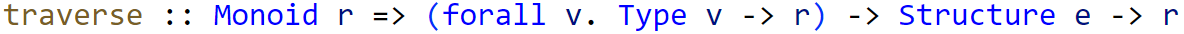
\includegraphics[scale=0.4]{CodeType18.png}
\end{figure}

A generic traversal of a structure is extremely powerful and the first step to a datatype-generic implementation.
The next step is traversing over the concrete values of a structure, which is only slightly more difficult.
Including an expression with the same type as the structure will refine both the expression and the structure when pattern matching.
It allows for functions to operate on fields within the datatype individually, but is restrictive in that it does not take in account the hierarchy it exists in.
A more involved traverse function makes available how a primitive type can be inserted and retrieved from the structure.

\begin{figure}[hbt!]
    \hspace{1em}
    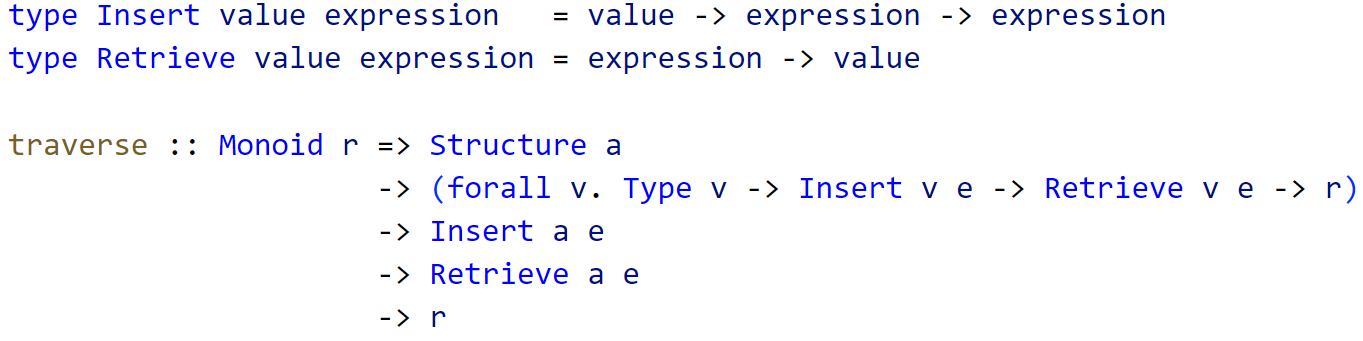
\includegraphics[scale=0.4]{CodeType19.png}
\end{figure}

The \type{Retrieve} function recursively accumulates the further we traverse into the structure.
The \type{Insert} function is slightly more involved, as it is recursive on the composed value.
Normally this would just be the input expression, but we are operating on the structure and do not have direct access to the actual expression.
Fortunately the \type{Retrieve} function is available to construct the expression to that point, which make the traversal function quite simple and compact.
To summarize, the \type{traverse} function creates two functions for each field within a datatype. 
One to insert a primitive type into the field, where the resulting expression will include the primitive type.
The other to extract the primitive type from the expression.
The \type{traverse} function can be used for various datatype-generic functions. 

\newpage

\paragraph{Intermediate}

The traversal function is the foundation for operating on two structures, required to construct and deconstruct variant types.
It is possible to create a mapping by traversing the other structure, and finding a specific primitive value.
This is both redundant and highly complex when considering that values must be removed from the available mappings once they have been matched.
The intermediate representation of a list, also used for computing the type representation, only requires a single traversal for each structure.
On the value-level it requires an heterogeneous list with all the different primitive types.
For this we use existential types, which allow type variables to be hidden and therefore be stored together.

\begin{figure}[hbt!]
    \hspace{1em}
    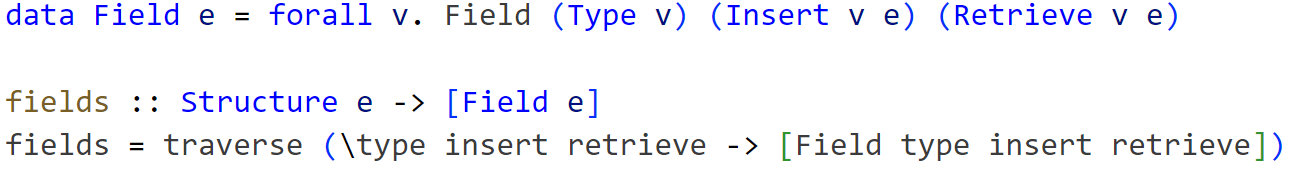
\includegraphics[scale=0.4]{CodeType20.png}
\end{figure}

Normally existential types result in functions not being able to discriminate between the hidden types.
As the primitive types exist within a GADT, pattern matching on the primitive type will reveal the type to the type system.
A structure can now be constructed or destructed by folding over such a list, but more importantly the fields can now easily be compared between structures.

\paragraph{Isomorphism}

The primary constraint is that the \type{construct} and \type{destruct} functions must be isomorphic from each other.
Both must map primitive types to the same fields, otherwise we cannot retrieve the same data from the representation.
It can be achieved by creating both mapping within the same function, such that all mapping decisions are inherently isomorphic.
This is trivial with the \type{Field} type, as we have access to functions that can insert and retrieve the value.
As example, a field in the variant (A) is chosen to be mapped to a field in the union (B).
The constructor can retrieve A and insert B, while the deconstructor would retrieve B and insert A.
Reinterpretation of the data can be incorporated when the fields are of different types.

\begin{figure}[hbt!]
    \hspace{1em}
    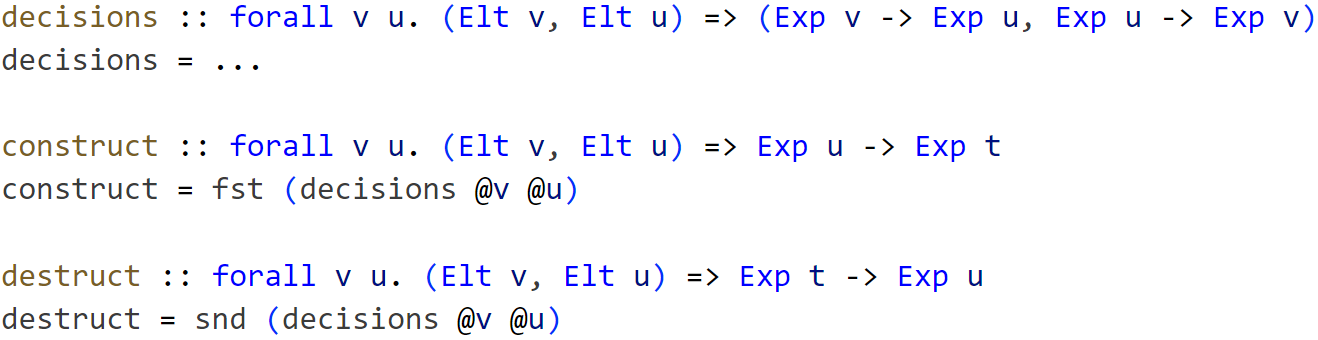
\includegraphics[scale=0.4]{CodeType21.png}
\end{figure}

It does mean that the constructor \type{v -> u} might make different decisions than the constructor \type{u -> v}, as decisions are made based from the perspective of one side. 
This is not a problem as constructed types must always be deconstructed first.
The union part of the \type{decisions} function is allowed to have spare fields, as they are the undefined fields within an union.

\paragraph{Steps}

To avoid a local optimum in the representation several iterations must be done within the \type{decisions} function.
A matching function determines whether there exist a mapping between two fields, and returns the functions that transform between the two primitive types.
This makes the decision function extensible, as long as the user specifies the relation between two fields.
Matching functions can be provided in order of preference.
An implementation can in some cases be made more efficient by sorting before matching, but this reduces the generality of the function. 
Some cases might require a custom \type{decisions} function, such as inserting multiple fields into a single field.
In general the implementation should be tailored to the implementation language.

\newpage

\section{Implementation}
In section \ref{type-level}, type-level was used to generate efficient representations for variant types.
In section \ref{datatype-generic}, mappings between representations are automatically created with datatype-generic programming.
It is sufficient to represent the initial sought after abstraction around variant types.
A collection can utilize the abstraction to represent variant types efficiently, depending on the circumstances.  

\begin{figure}[hbt!]
    \hspace{1em}
    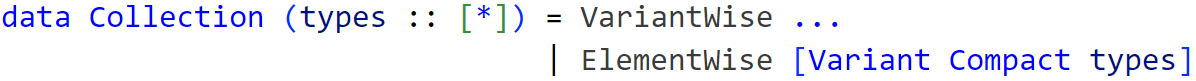
\includegraphics[scale=0.4]{CodeType22.png}
\end{figure}

While the implementation is heavily tailored to Haskell, it is not unfeasible to implement such a framework natively within a language.
This chapter centres around implementation details specific to Haskell and Accelerate.
In this first section Accelerate related details are explored, while the second section discusses the concrete implementation of (de)constructors.
The third section recuperates on the performance considerations and benchmarks the different approaches while maintaining the abstraction.

\subsection{Accelerate}

Accelerate is a data-parallel array language deeply embedded within Haskell.
An abstract syntax tree (AST) is created and optimized by Accelerate within Haskell's runtime system.
This greatly improves useability, as it can function as an Haskell library, at the cost of executing code within another runtime system.
The garbage collector of the Haskell runtime system is speculated to hinder performance\cite{accelerate-performance}. 
A type-safe interface to the compiler infrastructure LLVM enabled the creation of two backends: GPU and multi-core CPU's\cite{accelerate-llvm}. 
These backends can be used to execute a small set of collective operators in parallel; such as \type{map}, \type{fold} and \type{stencil}. 

\begin{figure}[hbt!]
    \hspace{1em}
    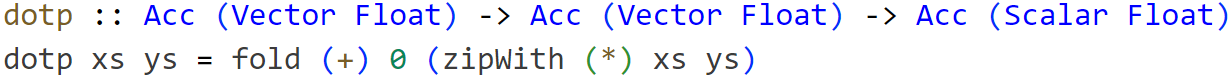
\includegraphics[scale=0.4]{CodeType23.png}
\end{figure}

The inherit thread-safety and fixed set of collective operators guarantee a consistent application of data-level parallelization.
It in addition allows for these collective operators to be heavily optimized in isolation, but also in relation to other collective operators.
A naive implementation of \type{dotp} would create an intermediate array for the results of the \type{zipWith} function\cite{accelerate-array-fusion}.
Fusing these operations would eliminate an iteration and the intermediate array, at the cost of potential register pressure. 
Accelerate fuses these collective operations, unless the fusion introduces duplicate work or the \type{compute} function is explicitly called.  
As Accelerate is embedded within Haskell, it uses algebraic data types and tuples for composite datatypes.
Datatypes must be {\it lifted} into the abstract syntax tree of Accelerate, which is implemented for all native types.
The \type{Exp} datatype represents the embedded representation.
User-defined datatypes can also be lifted into the AST with the previously discussed \type{Elt} class.
The notion of Algebraic Data Types does not exist within the embedded representation.

\begin{figure}[hbt!]
    \hspace{1em}
    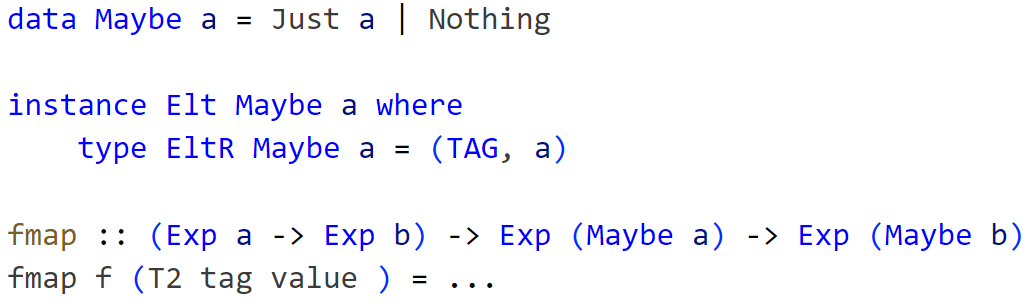
\includegraphics[scale=0.4]{CodeType24.png}
\end{figure}
\vspace{-0.5em}

The function retrieves the embedded \type{(TAG, Float)} type, not the sum type \type{MaybeFloat}.
Accelerate resolves this disconnection between surface and embedded representations through the use of {\it pattern synonyms}.

\paragraph{Pattern Synonymns}

A pattern synonym can be seen as an abstract constructor for a datatype.
While it is possible to achieve the same through regular functions, pattern synonyms also have the opportunity to act as a deconstructor.
Concretely it means pattern synonyms can been pattern matched against, which mean they act interchangeably to a normal datatype.
As pattern synonyms cannot share their name with their surface type an underscore is used to denote the difference. 
A limitation is that the compiler cannot prove the cases to be exhaustive, but completeness can be annotated with a compiler pragma.

\begin{figure}[hbt!]
    \hspace{1em}
    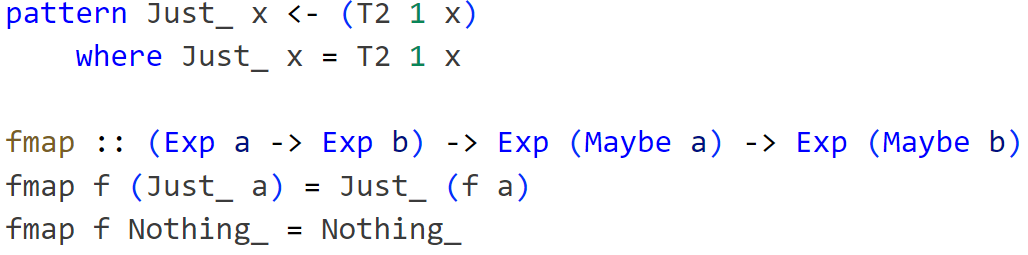
\includegraphics[scale=0.4]{CodeType25.png}
\end{figure}

It can be tedious to define pattern synonyms for all user defined datatypes, which is why Accelerate uses meta-programming to generate all constructors at compile-time.
Pattern synonyms can be extremely powerful and can be used to create a polymorphic constructor for our polymorphic variant type. 
Rather than a nominal constructor we use the position in the sum type, which can be statically constrained to be below the number of variants.
It can even be defined through a type-level natural number, but this requires type annotation for each use.
For useability the pattern synonyms \type{Con0, Con1,...} are defined to avoid the need for explicit type annotations.

\vspace{-0.2em}
\begin{figure}[hbt!]
    \hspace{1em}
    \includegraphics[scale=0.4]{CodeType26.png}
\end{figure}
\vspace{-0.2em}

In some cases it might be preferable to have a descriptive name, which can be done by creating a new pattern such as \type{pattern Nothing = Con1 ()}.
This will work on all sum types that have \type{()} as second data constructor, which one might consider to comprise type-safety.
The type can be constrained to only work for \type{Variant Compact [a, ()]}, but there cannot be any distinction between types that are composed similarly due to structural typing.  
A solution is to explicitly define a new datatype and derive all functionality through the variant type.

\paragraph{Pattern Matching}

Accelerate is deeply embedded within Haskell, which means a program effectively constructs an abstract syntax tree at the runtime of Haskell.
Pattern matching occurs while constructing the abstract syntax tree, which means we are effectively trimming the tree rather than extending it.
Stated more generally it is not possible to represent choice elements within a deeply embedded representation through the surface representation.
Explicit control flow is possible but Accelerate circumvents the restriction by explicitly defining all choice elements within a datatype.
When encountering a datatype with multiple choices, the function is repeatedly evaluated on a dummy type which contains the corresponding choice element.
Each deconstructor can therefore match only on the dummy type with the corresponding tag, which mean all possible branches can be obtained.
This is possible as pattern synonyms do not have to be isomorphic and the stub type is ignored within the Accelerate compiler.
As pattern matching cannot be overloaded in Haskell, the \type{match} operator is used to generate all choice elements recursively\cite{accelerate-pattern-matching}.

\newpage

\subsection{Result}

There are no setup requirements for using the variant type within Accelerate code.
Concretely, it is sufficient to use the \type{Variant} type constructor and the \type{Con0, Con1, Con2...} data constructors.
The expected behavior is that of a traditional sum type, where pattern matching happens on the current active variant. 
The intersect function discussed within the introduction only has to be written once, irregardless of any low level optimizations.
These optimizations include a variant type collection with multiple representations, multiple memory representations and efficient (de)constructor of variant types.
The \type{Primitive} and \type{Intersect} function, discussed in the introduction, can now be defined.

\begin{figure}[hbt!]
    \hspace{1em}
    \includegraphics[scale=0.4]{CodeType27.png}
\end{figure}

\vspace{-1em}

\paragraph{Memory Representation}

The \type{Compact} type already deduplicates primitive types of the same size, which makes the memory representation of \type{Primitive} already quite compact.
A more aggressive approach is to deduplicate on larger fields, which requires defining a type with the kind \type{[*] -> r}. 
Such type can be defined through pre-existing type-level functions, which can then be used as layout for all variant types.
The datatype-generic constructors adapt independently to the derived type and resort to truncation when deconstructing these fields.
As such, the \type{intersect} function does not have to adapt to a memory representation optimization.

\paragraph{(De)constructor}

The \type{Variant} type uses a single tag to represent the active variant, which is used by the \type{Case} operator to pattern match.
This is often quite performant, but in some cases it can be preferable to unconditionally execute a function.
The \type{Maybe} type can always unconditionally execute, as the \type{Nothing} constructor does not have any fields.
This is impossible with variant types that deduplicate fields, as unconditionally executing would impact used fields.
With the datatype-generic functions a bitmask can be unconditionally generated, which masks side-effects of all unconditionally executed functions.  
Rather than integrating this within the \type{Variant} type, it can be used as replacement for the pattern matching \type{match} operator.

\paragraph{Collection}

The datatype-generic functions allow for a collection of \type{Primitives} to be completely agnostic to the representation.
For a variant-wise collection pattern matching is redundant, which means to be effective all control-flow paths of the \type{intersect} function must be extracted. 
Pattern matching will effectively occur on the Haskell side, which is trivial due to embedded pattern matching already making choice elements explicit.
Distributing the \type{intersect} function over multiple arrays, within a collection of \type{Primitives}, can therefore be done.
With this many collective operations can be supported, including ones that modify the identity of such a collection.
These collective operators are currently not implemented beyond the necessary operators to support benchmarking.

\newpage

\subsection{Benchmarks}

A concrete performant way to operate on multiple variants was not the objective in its own right.
As discussed in the performance chapter, many components would be able to dictate the viability of a concrete optimization. 
In this section previously discussed optimizations are benchmarked, to demonstrate the viability of the abstraction around variant types.
The benchmarks will be done with the Criterion Haskell library, and will utilize both the multi-core CPU and GPU backend of Accelerate.
Benchmarks will be run on an {\it Intel Core i5-10600KF} CPU and a {\it NVIDIA GeForce RTX 3060 Ti} GPU.

\paragraph{Nearest}

The \type{nearest} function, the original motivating example, computes the nearest primitive that intersects with a ray.
The type of primitive include spheres, planes and triangles.
The Möller-Trumbore algorithm is used for the triangle intersection, while the plane and sphere use the obvious intersection algorithm.
In the benchmarks, a comparison is made with and between variant-wise collections.
The split category uses multiple functions for each primitive, and combines the results after.
The join category uses a single function, but branches on the index to determine the concrete primitive which is intersected with.
The element-wise collection are either randomly distributed or the primitives are grouped together to exploit potential coherence.
The compact representation deduplicates fields of equal size or smaller size, through the framework established in this thesis.
The benchmarks were run on 3000 equally distributed primitives, where the time in milliseconds is the average of 1000 samples.

\begin{center}
    \begin{tabular}{ | m{14em} | m{8em}| m{8em} | m{8em} | } 
      \hline
      {\bf Primitives: 3000} & {\bf CPU} & {\bf GPU} \\ 
      \hline
      Variant-wise split          & 4.76 ms & 1.11 ms\\ 
      \hline
      Variant-wise joined         & 4.17 ms & 0.74 ms\\ 
      \hline
      Random element-wise         & 4.32 ms & 0.77 ms\\ 
      \hline
      Sorted element-wise         & 4.32 ms & 0.77 ms\\ 
      \hline
      Compact random element-wise & 2.70 ms & 0.64 ms\\ 
      \hline
      Compact sorted element-wise & 2.70 ms & 0.63 ms\\ 
      \hline
    \end{tabular}
\end{center}

As seen in the results, the overhead of running multiple functions appears to exceed the cost of the branch on the primitive.
Scaling the amount of primitive intersection would give a more conclusive answer to whether it is actually faster and if the overhead can be recouped.  

\begin{center}
    \begin{tabular}{ | m{14em} | m{8em}| m{8em} | m{8em} | } 
      \hline
      {\bf Primitives: 300000} & {\bf CPU} & {\bf GPU} \\ 
      \hline
      Variant-wise split          & 5.06 ms & 1.73 ms\\ 
      \hline
      Variant-wise joined         & 4.69 ms & 1.10 ms\\ 
      \hline
      Random element-wise         & 5.01 ms & 1.12 ms\\ 
      \hline
      Sorted element-wise         & 4.86 ms & 1.10 ms\\ 
      \hline
      Compact random element-wise & 3.47 ms & 0.98 ms\\ 
      \hline
      Compact sorted element-wise & 3.39 ms & 0.95 ms\\ 
      \hline
    \end{tabular}
\end{center}

While it appears to recoup slightly for the multi-core CPU backend, the difference becomes larger for the GPU backend.
In general, the element-wise collections heavily benefit of the reduced memory footprint of the compact representations.
A surprise is that this does not translate to the joined category, which inherently uses the least amount of memory possible.
A possible explanation is that the non-contiguous memory and not being able to pattern match diminish the obtained benefit of using less memory.
This would also explain the discrepancy between multi-core CPU and GPU, as the difference is less significant on the GPU.
The large difference between the devices themselves can be most likely attributed to the inability of the CPU backend to vectorize the intersection algorithm.
This is unsurprising, as the control-flow within the individual intersections algorithms is complex and contains branches.  
The coherence of grouped primitives also has a minimal influence, which is likely a side-effect of the already unpredictable control-flow.
In summary, the framework but more specifically the deduplication algorithm appears to be useful and can be applied without changing existing architecture.

\newpage

\section{Discussion}

In this paper some fundamental choices have been made without extensive argumentation.
This chapter is used to highlight these choices and provide further reasoning for the choices that have been made.
It also highlights some limitations of the framework and ways these potentially can be resolved.

\subsection{Non-variant types}

In the preamble obtaining low-level control for datatypes in general was discussed.
The obtained method for variant types can be extended to product types, as it is effectively a simpler problem space.
Rather than deduplication, different padding strategies can be used to create multiple memory representations on the type-level.
The datatype-generic programming must be adapted to facilitate padding, which has already been previously discussed.
Ergonomic switching between representations can be achieved with a similar higher-kinded type constructor as \type{Variant}.

\begin{figure}[hbt!]
    \hspace{1em}
    \includegraphics[scale=0.4]{Discussion1.png}
\end{figure}
\vspace{-1em}

\subsection{Embedded Domain-Specific Language}

Libraries and domain-specific languages that are embedded construct their user-defined-types through the host-language.
A shallow embedding operates directly on types native to the host-language, while deep embeddings construct an abstract syntax tree that is later evaluated.
The latter offers flexibility on how user-defined types are implemented, as types exist both on the surface level and as construct within the abstract syntax tree.   
There are several approaches, which have been subject to research in the domain of circuit design.

\begin{itemize}
    \setlength\itemsep{0em}
    \item {C$\lambda$aSH} is not deeply embedded and operates on user-defined types through generics\cite{clash}. 
    \item Hydra has the deep embedding constructs nested into the shallow embedding constructs\cite{hydra}.
    \item Kansas Lava has both embeddings exist in parallel under an encasing type\cite{kansas-lava}.
    \item ForSyDe has both embeddings exist separately as standalone types\cite{forsyde}.
\end{itemize}

An observation is that user extendability is limited on deeply embedded constructs as execution models must be updated.
A proposed approach is to have a small deeply embedded core language that only supports constructs that are relevant for combinatorial optimizations\cite{shallow-and-deep}. 
The shallow embedding can be used to create an extensible and user-friendly interface to this core language.
In the context of data-parallel applications and variants this leans itself to an implementation in the host-language.
This distinction is irrelevant for languages that are not embedded in other languages.

\subsection{Datatype-generic programming in Haskell}

Current Accelerate derives the \type{Elt} class generically through Haskell's native datatype-generic framework.
It traverses the structure of the datatype, for each layer providing both the type and the transformation.
As these are intrinsically linked, deduplication must be represented both on the value-level and type-level.
The {\it Recursive Tagged Union}\cite{accelerate-sum-types} uses this approach, which proved to be problematic and complex.
One concern was that replacing the \type{Elt} class was considered to be a too invasive of an operation\cite{accelerate-sum-types}.
This means the \type{Elt} class must be derived from the implementation class, which limits user extendability. 
It is also not possible to sort the types on the type-level, as closed type families do not have an intrinsic link to its value-level construct.
An implementation that is fully modular and extendible on both the value-level and type-level prevent these complications.
Explicit derivation of the \type{Elt} class is also not required, as the sum type itself is effectively a polymorphic datatype that implements the \type{Elt} class. 

\newpage

\subsection{Limitations}

The framework has some limitations, either in general or specific to the implementation in Accelerate.
Within this section limitations will be discussed (further). 

\paragraph{Surface type}

As polymorphic variant types do not exist in Haskell, it is not apparent what the corresponding surface type should be.
Currently the raw memory representation is used, which might sound more problematic then it really is.
It means (de)constructing the variants must be done in the Accelerate code, rather than Haskell.
A solution can be to make a direct mapping to an existing extensible or open sum library.

\paragraph{Nested pattern matching}

Since tags are statically determined for each type individually, nested pattern matching is not trivial. 
Currently the datatype \type{TagR} is used, where \type{Just (Just a)} is represented as \type{TagRtag 1 (TagRtag 1 (TagRsingle a))}. 
Pattern matching on the first \type{Just} would remove one layer, and the rest is propagated along.

\begin{figure}[hbt!]
    \hspace{1em}
    \includegraphics[scale=0.4]{Discussion2.png}
\end{figure}

An important detail is that these tags are generated statically, for all possible permutations.
In a type with deduplicated fields the {\it nested} datatype is not necessarily available, as it might be constructed through different fields.
As the \type{TagR} is constrained to the same structure as the encapsulating type, it is not possible to list all possible permutations through the \type{TagR} type.
A solution is to just lose the constraint on the \type{TagR} type, and allow for more flexibility.
As the \type{TagR} type is integrated with the \type{Elt} class, a change would require some changes to existing Accelerate code.

\paragraph{Unified tag}

An extension of the previous discussion is the use of a single tag, for multiple nested tags.
It involves operations to extract and construct the tag, which can be computationally expensive.
Currently the deduplication algorithm has no knowledge of tags at all, and sees them as any other field.
An implementation would complicate both the deduplication process and automatic derivation of (de)constructors.
A temporary solution would involve simply flattening the sum type, which would also be more performant in the general case.
Another solution would be to change perspective and argue tags are datatypes with a fixed size depending on the amount of choices they represent.
Both the type-level and datatype-generic part could handle tags as any other fields, and can upscale them to an existing datatype.

\paragraph{Struct}

While it possible to derive struct-like memory representations, Accelerate does not (yet) have the instructions to insert and extract those values.
As primitive types are implicitly distributed over multiple arrays, there is no need to operate on a type within a larger type. 
It in addition does not allow types existing outside the predefined types, which means memory representation is limited to that set of types.
A solution would be to add an (untyped) type with a variable size and corresponding instructions to extract (aligned) data.

\paragraph{Compilation Speed}

As type-level programming is done statically, it puts additional strain on the compilation speed of programs.
This might become apparent in larger projects, where statically resolving many interactions might become too costly.
It also exists for the datatype-generic programming part, as data (de)constructors {\it might} recompute the mapping each time.
Strictly speaking it can be optimized away, but this might not always be obvious to the compiler. 
This is less of an issue for embedded languages, as it occurs while constructing the abstract syntax tree. 

\newpage

\section{Conclusion}

The first research question of this thesis was:

\begin{quote}
{\it How to obtain low-level control that is applicable for high performance computing, while preserving the higher-abstraction surface representation?}
\end{quote}

Answering this required understanding performance implications of low-level optimizations, an exposition of relevant considerations was therefore done in the first chapter of this thesis.
The importance of contiguous memory allocation, cache efficiency, access patterns and influence of branching was demonstrated.
Due to the inability to derive an efficient solution from a mere theoretical framework, the flexibility of representations became prominent in the task to capture low-level control.  
This thought was used for answering the second research question of this thesis:

\begin{quote}
{\it What is the conceptualization of a higher-abstraction variant type, which can exercise the obtained low-level control within in a data-parallel environment?}
\end{quote}

A polymorphic variant type was used, which is able to represent both element-wise and variant-wise collections.
It also gave the opportunity to use type-level programming for a deduplicating algorithm for variant types, which can be extended by the user.
Datatype-generic was successfully used to create isomorphic mappings between datatypes, which made data (de)constructors independent of the concrete memory representation.
As such a fully modular framework has been established, which can capture various low-level optimizations through a higher-abstraction variant type.
An implementation was realized in Accelerate, an embedded domain-specific data-parallel language in Haskell, which demonstrates the viability of the established flexibility.
Concretely, the low-level control of the second research question has been obtained through polymorphic variant types that are flexible in their memory representation.
It creates the foundation for answering the first research question, where low-level control has been established through type-level and datatype-generic programming. 

\subsection{Future Work}

Within this thesis a notable focus was the performance of predictable non-uniformity, which is data that is not dependant on a previous computation.
Exceptions in particular are not predictable, and as such must use an element-wise collection.
It can be more performant to effectively filter out the exception states, that is the transform from an element-wise collection to an variant-wise collection.
It would require a performant data-parallel grouping algorithm, which is not trivial to implement and as such subject to future research.
It can be categorized together with other applications that can potentially accelerate operations in specific use case, such as task-parallelism. 

\newpage

\newgeometry{margin = 2cm}

\bibliographystyle{abbrv}
\bibliography{refs}

\end{document}